\documentclass[thesis=B,czech]{FITthesis}[2012/06/26]

\usepackage[utf8]{inputenc}
\usepackage{graphicx}
\usepackage{dirtree}
\usepackage{float}
\usepackage{color}
\usepackage{listings}

\lstdefinelanguage{RainerScript}
{
  morekeywords={
    module, if, then, while, for, load, set, unset,
	template, name, type, string, action, stop, and,
    from, to, var, stringtobedeleted, severity, target,
    port, protocol, contains, else, queue, dequeueslowdown,
    dequeuebatchsize, size
  },
  sensitive=false,
  morecomment=[l]{\#},
  morecomment=[s]{/*}{*/},
  morestring=[b]"
}

\lstdefinelanguage{PKGBuild}
{
  morekeywords={
    pkgname, pkgver, arch, depends, source, md5sums,
    build, package, pkgdir
  },
  sensitive=false,
  morecomment=[l]{\#},
  morecomment=[s]{/*}{*/},
  morestring=[b]"
}

\lstdefinelanguage{Ash}
{
  morekeywords={
    if, fi, then, else, exit, return, echo, time, rm, awk, grep,
    cat, tr, cut, for, in, do, done
  },
  sensitive=false,
  morecomment=[l]{\#},
  morecomment=[s]{/*}{*/},
  morestring=[b]"
}

\lstdefinestyle{AshStyle} %{language=Bash,style=numbers,style=MyFrame,frame=none,backgroundcolor={}}
{language=Ash,                % choose the language of the code
basicstyle=\footnotesize,       % the size of the fonts that are used for the code
numbers=left,                   % where to put the line-numbers
numberstyle=\footnotesize,      % the size of the fonts that are used for the line-numbers
stepnumber=1,                   % the step between two line-numbers. If it is 1 each line will be numbered
numbersep=5pt,                  % how far the line-numbers are from the code
backgroundcolor=\color{white},  % choose the background color. You must add \usepackage{color}
showspaces=false,               % show spaces adding particular underscores
showstringspaces=false,         % underline spaces within strings
showtabs=false,                 % show tabs within strings adding particular underscores
frame=single,           % adds a frame around the code
tabsize=2,          % sets default tabsize to 2 spaces
captionpos=b,           % sets the caption-position to bottom
breaklines=true,        % sets automatic line breaking
breakatwhitespace=false,    % sets if automatic breaks should only happen at whitespace
escapeinside={\%*}{*)}          % if you want to add a comment within your code
}

\lstdefinestyle{RainerScriptSimpleStyle} %{language=Bash,style=numbers,style=MyFrame,frame=none,backgroundcolor={}}
{language=RainerScript,                % choose the language of the code
basicstyle=\footnotesize,       % the size of the fonts that are used for the code
backgroundcolor=\color{white},  % choose the background color. You must add \usepackage{color}
showspaces=false,               % show spaces adding particular underscores
showstringspaces=false,         % underline spaces within strings
showtabs=false,                 % show tabs within strings adding particular underscores
frame=lines,           % adds a frame around the code
tabsize=2,          % sets default tabsize to 2 spaces
captionpos=b,           % sets the caption-position to bottom
breaklines=true,        % sets automatic line breaking
breakatwhitespace=false,    % sets if automatic breaks should only happen at whitespace
escapeinside={\%*}{*)}          % if you want to add a comment within your code
}

\lstdefinestyle{RainerScriptStyle} %{language=Bash,style=numbers,style=MyFrame,frame=none,backgroundcolor={}}
{language=RainerScript,                % choose the language of the code
basicstyle=\footnotesize,       % the size of the fonts that are used for the code
numbers=left,                   % where to put the line-numbers
numberstyle=\footnotesize,      % the size of the fonts that are used for the line-numbers
stepnumber=1,                   % the step between two line-numbers. If it is 1 each line will be numbered
numbersep=5pt,                  % how far the line-numbers are from the code
backgroundcolor=\color{white},  % choose the background color. You must add \usepackage{color}
showspaces=false,               % show spaces adding particular underscores
showstringspaces=false,         % underline spaces within strings
showtabs=false,                 % show tabs within strings adding particular underscores
frame=single,           % adds a frame around the code
tabsize=2,          % sets default tabsize to 2 spaces
captionpos=b,           % sets the caption-position to bottom
breaklines=true,        % sets automatic line breaking
breakatwhitespace=false,    % sets if automatic breaks should only happen at whitespace
escapeinside={\%*}{*)}          % if you want to add a comment within your code
}

\lstdefinestyle{PKGBuildStyle} %{language=Bash,style=numbers,style=MyFrame,frame=none,backgroundcolor={}}
{language=PKGBuild,                % choose the language of the code
basicstyle=\footnotesize,       % the size of the fonts that are used for the code
numbers=left,                   % where to put the line-numbers
numberstyle=\footnotesize,      % the size of the fonts that are used for the line-numbers
stepnumber=1,                   % the step between two line-numbers. If it is 1 each line will be numbered
numbersep=5pt,                  % how far the line-numbers are from the code
backgroundcolor=\color{white},  % choose the background color. You must add \usepackage{color}
showspaces=false,               % show spaces adding particular underscores
showstringspaces=false,         % underline spaces within strings
showtabs=false,                 % show tabs within strings adding particular underscores
frame=single,           % adds a frame around the code
tabsize=2,          % sets default tabsize to 2 spaces
captionpos=b,           % sets the caption-position to bottom
breaklines=true,        % sets automatic line breaking
breakatwhitespace=false,    % sets if automatic breaks should only happen at whitespace
escapeinside={\%*}{*)}          % if you want to add a comment within your code
}

\department{Katedra softwarového inženýrství}
\title{Flexibilní logování pro embedded Linuxové systémy}
\authorGN{David}
\authorFN{Vavřička}
\authorWithDegrees{David Vavřička}
\supervisor{Ing. Matěj Laitl}
\acknowledgements{Na tomto místě bych rád poděkoval a vyslovil uznání Maťeji Laitlovi, vedoucímu mé bakalářské práce, za správné směrování, cenné rady a řešení otázek, se kterými jsem se na něj obracel. 

Dále děkuji firmě Nangu.TV za umožnění vzniku této bakalářské práce. }
\abstractCS{Tato bakalářská práce se zabývá analýzou, návrhem a následnou implementací nového logovacího řešení pro set-top box EKT DID7006mTF.

Hlavním cílem je přepracovat současné logovací řešení a přidat mu podporu vzdáleně měnit jeho konfiguraci, a umožnit tak snížit vytížení sítě.

Na základě analýzy byl nasazen logovací démon Rsyslog, pro nějž byli naprogramovány dva moduly, dále bylo naprogramováno API umožňující změnu konfigurace logování a byly napsány podpůrné skripty.

V závěru práce bylo nové řešení otestováno na reálném hardware, čímž bylo demonstrováno splnění požadavků a příznivé provozní vlastnosti.}
\abstractEN{This Bachelor’s thesis deals with analysis, design and implementation of a new logging solution for EKT DID7006mTF set-top box.

The main goal of this thesis is to redesign the current logging solution and to add functionality to change logging configuration remotely to allow to reduce amount of network load.

Based on the results of the analysis Rsyslog logging daemon was deployed and two Rsyslog modules were developed, in addition a new API for configuration change and some subsidiary scripts were developed as well.

The new solution was tested on real hardware where accomplishment of all desired goals and good running characteristics were demonstrated.}
\placeForDeclarationOfAuthenticity{V~Praze}
\declarationOfAuthenticityOption{4} %volba Prohlášení (číslo 1-6)
\keywordsCS{logování zpráv, logovací démoni, Rsyslog, set-top boxy, vestavěné systémy, Linux}
\keywordsEN{message logging, logging daemons, Rsyslog, set-top boxes, embedded systems, Linux}

\begin{document}

\begin{introduction}
Zadavatelem práce je společnost vyvíjející set-top boxy pro sledování internetové televize, která prodává hotová řešení pro IPTV streaming jednotlivým provozovatelům.

V současné době využívají služeb provozovatelů desetitisíce zákazníků, a trend ukazuje, že se jejich počet bude do budoucna nadále zvyšovat.

Každý ze set-top boxů v domácnostech uživatelů odesíla stovky zpráv za minutu o svém stavu na servery jednotlivých provozovatelů. Jejich zpracování představuje pro servery velkou zátěž, dále zprávy mohou zahltit už tak vytíženou linku ve směru od uživatele, a proto byl sepsán seznam technických požadavků, jež si kladou za cíl umožnit snížit objem logů posílaných na servery.

Tato práce se ve své první části zabývá analýzou technických požadavků a výběrem vhodného postupu řešení.
 
Na základě analýzy je posléze provedena implementace, ve které je kladen důraz na použití pouze volně šířitelných open-source projektů a jejich případné rozšíření.
 
V závěru práce je výsledné řešení podrobeno testovaní, kde se kromě splnění technických požadavků zkoumají z důvodu omezeného výkonu set-top boxů nároky na výpočetní výkon.
\end{introduction}

\chapter{Technické požadavky}
Cílem je upravit logovací řešení pro set-top box EKT DID7006mTF~\cite{ekt7006} tak, aby splňovalo technické požadavky popsané v této kapitole. Řešení musí fungovat a být otestováno na zmíněném modelu set-top boxu, a pokud možno, mělo by být přenositelné i na jiné typy set-top boxů.

Původním záměrem bylo rozdělit požadavky na základní a rozšířené. Nakonec zadavatel rozhodl, že všechny níže zmíněné požadavky jsou základní, a tedy jejich implementace je nutná pro splnění práce.

\section*{Snížení objemu logů}
Cílem tohoto požadavku je umožnit snížit objem zasílaných logů z důvodu přílišného zatížení sítě a serverových disků. A to tak, že zadavatel bude schopen nadefinovat pro každou komponentu úroveň severity zpráv, od které mají být posílány na server. Výchozí nastavení dodá zadavetel.

\section*{Vzdálená konfigurace}
Řešitel navrhne API, jež umožní za běhu měnit maximální severitu zpráv pro jednotlivé komponenty, a dále toto API musí umožňovat nastavit výchozí severitu, která se použije pro komponenty, jež ji nemají explicitně nastavenou. Takto změněné nastavení musí být perzistentní i po restartu STB. Výchozí nastavení se obnoví až po factory resetu.

\section*{Rate-limiting odesílaných zpráv}
Nové logovací řešení musí být schopné provádět rate-limiting odesílanych zpráv tak, aby nepřekročilo maximální vyhrazenou šířku pásma. Naivní rate-limiting je i v existujícím řešení. Řešitel navrhne výchozí nastavení nového řešení tak, aby přibližně odpovídalo původnímu chování. 

\section*{Formát logů}
Je nutno zachovat formát logů jako ho má původní řešení, aby se jednalo o drop-in replacement bez nutnosti jakkoli měnit konfiguraci serveru, který sbírá logy od set-top boxů.

\section*{Razítkování zpráv}
Každé zprávě se musí přidat textový prefix id=N, kde N monotonicky roste s každou zprávou.  To slouží pro detekci ztracených zpráv. Id přeteče po dvaceti bitech. Po rebootu STB id znovu začíná od jedné.

\section*{Post-processing zpráv}
Zadavatel má pouze částečnou kontrolu nad zprávami generovanými aplikacemi na set-top boxu, například nedokáže ve všech případech eliminovat dlouhé prefixy u zpráv. Je proto nutno takové prefixy rozpoznat, a vhodně odfiltrovat před odesláním. Ze stejného důvodu mají některé zprávy nevhodně vyplněnou severitu a položku app-name. Jejich správné hodnoty jsou uloženy v textu zprávy, jejíž formát je pro jednotlivé skupiny zpráv konstantní. Řešení bude schopné tyto údaje z těla zprávy extrahovat, a nahradit jimi původní metadata.
 
Řešitel vytvoří pro ukázku tři pravidla, která budou sloužit zadavateli jako šablony pro možná budoucí filtrovací pravidla. Tato pravidla musí být možné definovat a měnit bez nutnosti nového sestavení softwaru.

\chapter{Logování v linuxových systémech}
Systém a aplikace na něm běžící informují o svém stavu prostřednictvím zpráv, jež jsou užitečné pro získání statistických údajů, k ladění programů nebo např. pro detekování útoků.

Je užitečné, aby zprávy měly unifikovaný formát, a aby byl jednoznačně určen způsob jejich přenosu po síti. To na unixových, a tedy i linuxových systémech specifikuje protokol Syslog.

Dále je ku prospěchu věci zprávy centralizovaně zachytávat a spravovat, k čemuž slouží tzv. logovací démon. 

\section{Logovací démon}
Démon je v unixovém světě označení pro takový proces, který oproti běžným procesům neintereaguje přímo s uživatelem, ale běží na pozadí operačního systému a funguje samostatně. Hlavním účelem logovacího démona je sběr logů od ostatních procesů, které následně v závislosti na jeho konfiguraci dokáže filtrovat a ukládat na disk či odesílat na vzdálený server.

\section{Protokol Syslog}
Protokol Syslog~\cite{NetworkAdmSurGuide} spatřil světlo světa již v roce 1980. Má ho na svědomí Eric Allman, který jej psal s úmyslem využít ho pro potřeby projektu Sendmail. Nicméně postupem času byl tento protokol díky skvělému návrhu a díky své jednoduchosti adaptován i jinými projekty. Rozšířil se na různé OS, a později se stal standardem pro logování na většině Unixových systémů.

Protokol především specifikuje podobu zpráv a způsob jejich přenosu po síti.

\subsection{The BSD syslog Protocol - RFC 3164}
Až přibližně po dvaceti letech od vzniku protokolu Syslog sepsal (v roce 2001) Chris Lonvick dokument RFC~3146~\cite{RFC3164} popisující daný protokol. Do té doby existovala velká spousta v detailech se lišících implementací, což mělo v jistých případech za následek nekompatibilitu.

Ještě v dnešní době je možno nalézt systémy s logovacím řešením, které specifikuje tento dokument. Nicméně čím dál častěji je nahrazován svým následníkem, kterým je RFC 5424.

\subsection{The Syslog Protocol - RFC 5424}
Oficiální standard specifikující protokol Syslog vznikl až s příchodem protokolu RFC 5424, který světu představil v roce 2009 jeho autor Rainer Gerhards. Došlo v něm k některým zásadním a velice užitečným změnám.

Nový standard umožňuje použití libovolného trasnportního protokolu~\cite{RFC5424-TrProt} oproti RFC 3164, kde je jako transportní protokol pevně určeno UDP~\cite{RFC3164-UDP}.
Změn doznal také formát zpráv, který již nemá jen jednu pevně danou podobu, ale je možno jej přispůsobit dle specifických potřeb~\cite{RFC5424-MsgForm}. To má ovšem za následek zpětnou nekompatibilitu s RFC~3164.

\section{Formát zpráv}
\begin{figure}[H]
	\centering
	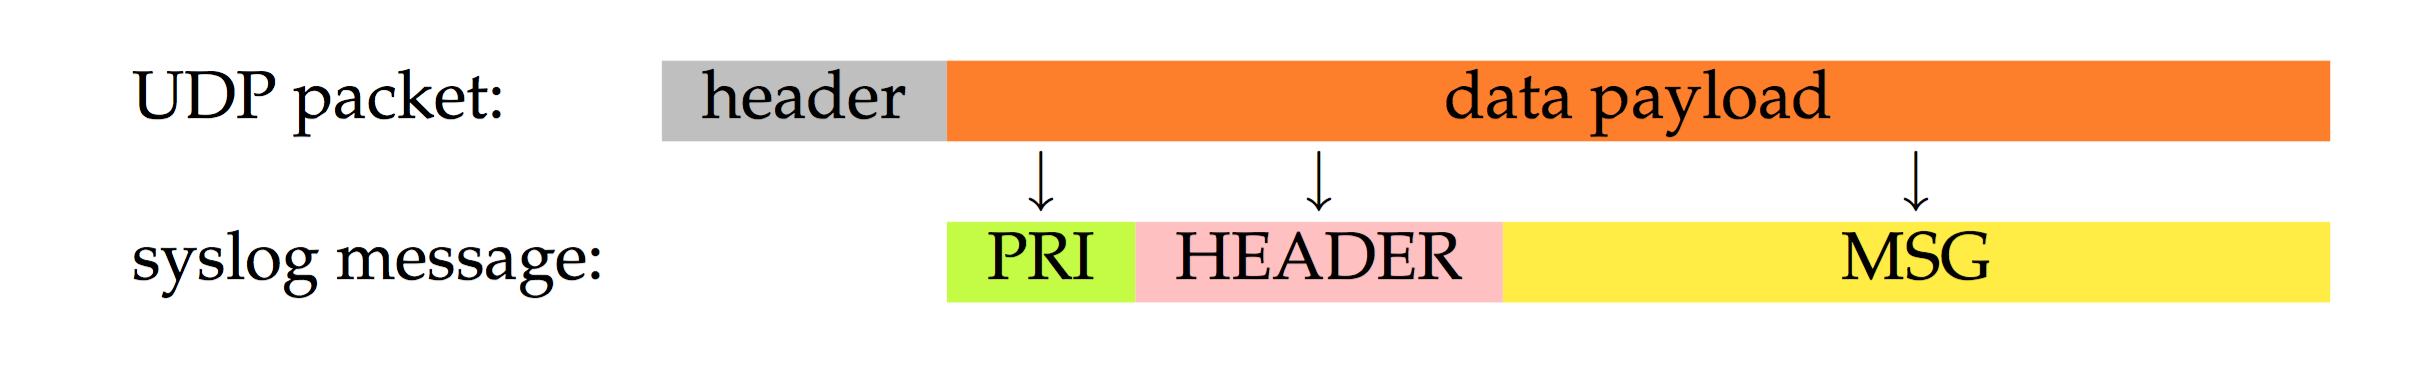
\includegraphics[scale=0.3]{images/syslog-message-format}
	\caption[Formát zpráv dle RFC 3164 a RFC 5424]{Formát zpráv dle RFC 3164 a RFC 5424}
\end{figure}

Zpráva se skládá ze tří částí, jak je pro lepší představu graficky vyzobrazeno na obrázku 2.1.

\subsection{Část PRI}
PRI se skládá z jedno- až tří-místného decimálního čísla PRIVAL ohraničeného symboly~\uv{<}~na začátku a~\uv{>}~na konci.
PRIVAL má v sobě zakódované číselné hodnoty parametrů zprávy označovaných jako Severity a Facility.
$$Prival= 8*Facility+Severity$$
Facility určuje zdroj logů a Severity jejich důležitost (tedy zda se jedná např. pouze o ladící zprávu, nebo naopak o důležitou zprávu např. o pádu programu).
\clearpage
Na základě těchto dvou hodnot logovací démon provádí základní filtraci zpráv.
Důležitým poznatkem je, že formát PRI je shodný podle dokumentů RFC~5424 i RFC~3164.

\begin{table}[ht]
\centering
	\caption[Tabulka severit dle RFC~3164]{Seznam severit dle RFC~3164.~\cite{RFC3164}}
	\begin{tabular}{|l|l|l|}\hline
		Číselný kód	& Severity & Význam	\tabularnewline \hline \hline
		0		& Emergency	&	Systém je nepoužitelný \tabularnewline \hline
		1		& Alert		&	Vyžadována okamžitá reakce \tabularnewline \hline
		2		& Critical	&	Kritický stav \tabularnewline \hline
		3		& Error		&	Chybový stav	\tabularnewline \hline
		4		& Warning	&	Upozornění na hrozící chybu \tabularnewline \hline
		5		& Notice		&	Neobvyklý stav, ale ne chybový \tabularnewline \hline
		6		& Informational & Informační zpráva \tabularnewline \hline
		7		& Debug		&	Ladící zpráva \tabularnewline \hline
	\end{tabular}
\end{table}

\begin{table}[ht]   %[H] místo [ht] aby to bylo přesně na daném místě
\centering
	\caption[Tabulka facilit dle RFC~3164]{Seznam facilit dle RFC~3164.~\cite{RFC3164}}
	\begin{tabular}{|l|l|l|}\hline
		Číselný kód & Facility & Původ zpráv \tabularnewline \hline \hline
		0		& kern & Zprávy jádra systému	\tabularnewline \hline
		1		& user & Generované uživatelem	\tabularnewline \hline
		2		& mail & Generované emailovým systémem			\tabularnewline \hline
		3		& daemon & Systémoví démoni			\tabularnewline \hline
		4		& auth & Zprávy autorizačního charakteru		\tabularnewline \hline
		5		& syslog & Generované syslogem	\tabularnewline \hline
		6		& lpr & Tiskový systém		\tabularnewline \hline
		7		& news & Network news systém		\tabularnewline \hline
		8		& uucp & UUCP systém			\tabularnewline \hline
		9		& cron & Zprávy plánovacího systému Cron			\tabularnewline \hline
		10		& security & Zprávy zabezpečovacího charakteru	 \tabularnewline \hline
		11		& ftp & FTP démon				\tabularnewline \hline
		12		& ntp & NTP systém			\tabularnewline \hline
		13		& logaudit & Log audit				\tabularnewline \hline
		14		& logalert & Log alert				\tabularnewline \hline
		15		& clock & Clock démon			\tabularnewline \hline
		16		& local0 & Lokální zprávy (0)			\tabularnewline \hline
		17		& local1 & Lokální zprávy (1)			\tabularnewline \hline
		\ldots	& \ldots				\tabularnewline \hline
		23		& local7 & Lokální zprávy (7)			\tabularnewline \hline
	\end{tabular}
\end{table}

\subsection{Header}
Tato část zprávy obsahuje časovou značku a identifikaci zdroje (podle IP adresy nebo hostname). Přesnou podobu Headeru specifikují dokumenty RFC~3164 a RFC~5424 odlišně. Zatímco starší dokument definuje přesnou podobu časové značky, tak novější specifikace dovoluje různé formáty. Díky tomu není zaručena plná zpětná kompatibilita.

\subsection{MSG}
Část Msg pokrývá zbývající část zprávy. Jejím obsahem jsou různé zbývající informace o procesu generujícího danou zprávu a pak samozřejmě samotný text zprávy.

\chapter{Analýza}
V úvodu kapitoly je popsán STB a na něm běžící pro tuto práci důležité aplikace.
Následuje popis infrastuktury (vyjádřený formou diagramu na obr. 3.1), kde je znázorněna komunikace mezi STB a servery zadavatele.
Kapitolu zakončuje analýza řešení jednotlivých technických požadavků a srovnání logovacích démonů.

\section{Původní řešení}
\begin{figure}[ht]
	\centering
	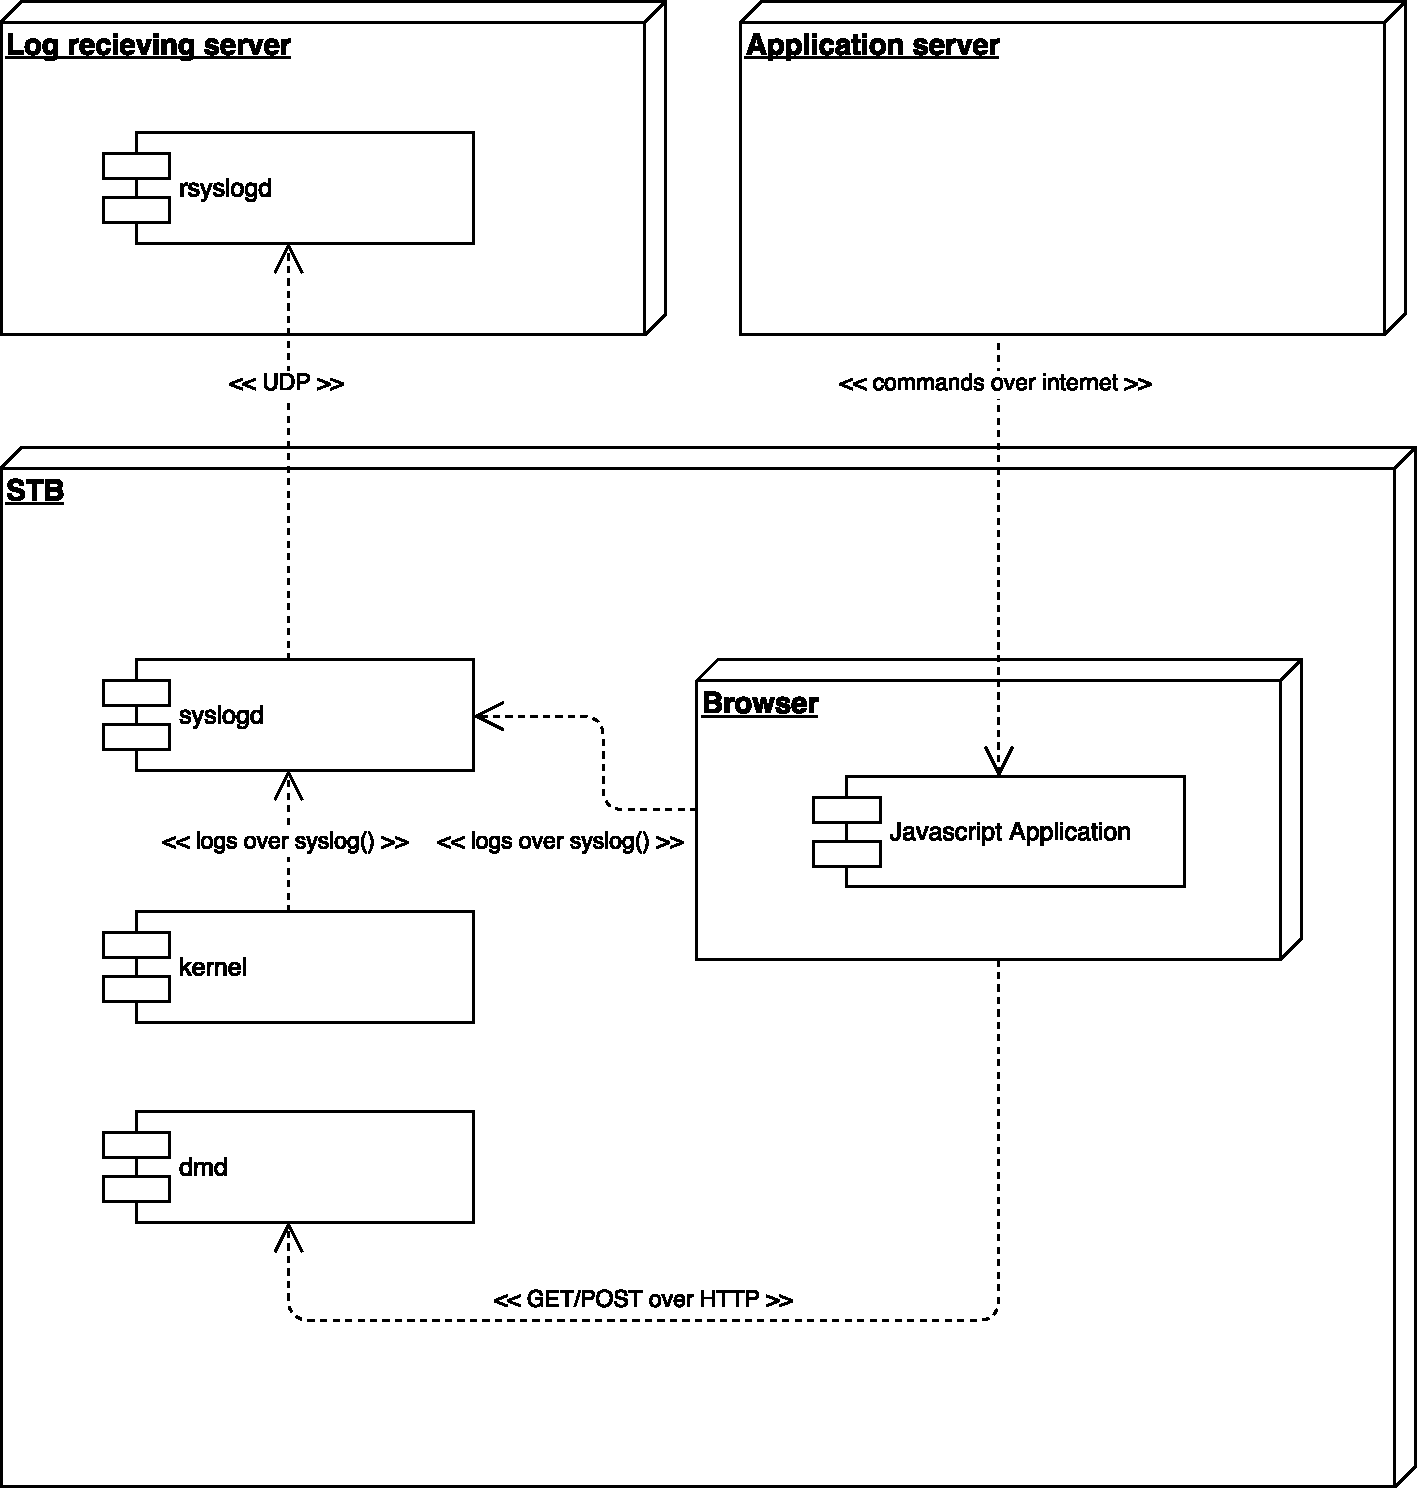
\includegraphics[scale=0.5]{images/diagram-puvodniho-reseni}
	\caption[Diagram původního řešení]{Diagram původního řešení}
\end{figure}

\subsection{HW specifikace STB EKT DID7006}
\begin{description}
\setlength\itemsep{-1ex}
  \item [CPU:] ARM 9 Ali M3733 (1GHz Dual core)
  \item [GPU:] Mali 400
  \item [RAM:] 512MB DDR3
  \item [Perzistentní paměť:] 512MB NAND Flash
\end{description}

\subsection{Runtime prostředí}
Na STB běží OS GNU/Linux se sadou aplikací BusyBox, která nahrazuje standardní shellové utility GNU. Aplikace BusyBoxu jsou díky své malé velikosti vhodnější pro embedded zařízení. Na druhou stranu neposkytují všechny funkce a možnosti nastavení plnohodnotných GNU Core Utilities.

\subsubsection{Browser}
Browser je jednoduchý internetový prohlížeč dodaný výrobcem STB.
V něm běží v JavaScriptu zadavatelem napsaná aplikace poskytující uživatelské rozhraní. Mimo to také naslouchá zprávám z aplikačního serveru, na jejichž základě může provádět akce, a to včetně generování POST či GET requestů pro démona Dmd.
Tato JavaScriptová aplikace spolu s dalším podpogramem nesoucím název Player generují velké množství logů. Tyto logy nepoužívají standardizovanou množinu severit dle dokumentu RFC 3164, ale svou vlastní s ní nekompatibilní. Logovací démon ovšem očekává zprávy právě podle standardu zmíněného dokumentu. Implementaci Browseru ani Playeru nemůže zadavatel měnit a proto je třeba nekompatibilitu vyřešit pomocí logovacího démona.

\subsubsection{Servisní komponenta Dmd}
Dmd je v C++ napsaná servisní komponenta, která zprostředkovává komunikaci mezi Browserem a shellovým prostředím pomocí minimalistického HTTP serveru.
Na základě dotazů GET a POST dokáže spouštět shellové příkazy, a bude možné ji tak v budoucnu využít jako prostředníka k volání funkcí v této práci naprogramovaného API.

\subsubsection{BusyBox Syslogd}
Jedná se o minimalistického logovacího démona, který je podrobněji popsán v oddílu \uv{Srovnání logovacích démonů}.
Zadavatel mu pro své potřeby navíc doimplementoval číslování jednotlivých zpráv pro rozpoznání výpadku a za druhé naivní rate-limiting zpráv. Ten je naivní z důvodu, že používá statický buffer na počet zpráv, který nebere ohled na jejich velikost, a hlavně bufferované zprávy se neodešlou samy, ale jen s nově příchozími zprávami.
Za použití tohoto démona není možné splnit některé stěžejní technické požadavky, jako například \uv{Snížení objemu logů} nebo \uv{Post processing zpráv}. Proto bude nutné ho nahradit nějakým vyspělejším démonem. Tím se ale zabývá až další oddíl \uv{Nové řešení}.

\subsection{Aplikační server}
Aplikační server se stará o business logiku, například poskytuje uživateli práva přehrát daný kanál nebo film, komunikuje s JavaScriptovou aplikací, která se vůči němu autorizuje a podobně.
AS není možné v této práci jakkoli měnit a je nutné zachovat kompatibilitu.

\subsection{Servery pro sběr logů}
Provozovatel vlastní cluster serverů pro sběř logů od desetitisíců STB. Běží na nich logovací démon Rsyslog nakonfigurovaný pro co nejvyšší propustnost. Stejně jako v případě AS, není v této práci možné měnit jeho implementaci.

\section{Nové řešení}
Prvně je nutno zvážit, zda problém řešit na straně serveru nebo set-top boxu. Vhodnou konfigurací logovacího démona na straně serveru, který by nepotřebné zprávy zavčas rozpoznal, zahodil a dále nezpracovával, by bylo možné splnit požadavek na snížení zátěže serverových disků. Přetížení sítě se takto vyřešit ale nedá, a proto bylo toto řešení zavrhnuto.

Je tedy nutno problém řešit na straně set-top boxu, kde je původní řešení postaveno na BusyBox Syslogd. Nabízí se možnost upravit fungování tím způsobem, aby se logy s nízkou severitou už na set-top boxu zahazovaly, a pouze v případě potřeby bylo umožněné na dálku změnit konfiguraci démona tak, aby se povolilo logování pro zprávy s nastavenou danou komponentou a severitou. Takovou možnost prostý Syslogd neposkytuje (stejně jako neumožňuje splnění většiny vytyčených technických požadavků práce), a je proto nutno zvážit napsání vlastního démona, nasazení jiného (vyspělejšího) logovacího démona nebo rozšíření stávajícího démona Syslogd.

\subsection{Srovnání logovacích démonů}
V tomto oddílu jsou popsáni vybraní logovací démoni a v jejím závěru jsou porovnáni.
\subsubsection{BusyBox Syslogd}
Tato logovací utilita se skládá ze dvou démonů, jmenovitě z Klogd, který zachytává logy z kernelu a předává je ke zpracování démonu Syslogd. Syslogd pak zachytává i všechny zbylé zprávy a dále s nimi nakládá. Má však velice omezený rozsah schopností. Dokáže pouze zprávy lokálně ukládat, přeposílat je dále po síti, zahazovat duplikáty, rotovat zprávy v závislosti na velikosti a filtrovat je podle omezených kritérií. Dokáže totiž filtrovat zprávy pouze podle typu facility, a už nikoli podle názvu komponenty, která ji vygenerovala.

\subsubsection{Syslog-ng}
Syslog-ng je flexibilní logovací démon zaměřený na centralizované a zabezpečené logování. Má široké možnosti nastavení a poskytuje množství funkcí. Takže jeho vhodným nakonfigurováním se dá snadno splnit většina vytyčených technických požadavků~\cite{syslogNg}, až na požadavky na vzdálenou změnu konfigurace a změnu severity zpráv.

\subsubsection{Rsyslog}
Výčet funkcí Rsyslogu je ještě obsáhlejší než u Syslog-ng~\cite{Rsyslog-features}. Technické požadavky se s jeho použitím tedy také dají splnit všechny, kromě vzdálené změny konfigurace a post-processingu zpráv. Stejně jako Syslog-ng není jen logovacím démonem, ale i analyzérem zpráv. Dokáže tak zprávy podle jejich obsahu měnit, třídit a jinak s nimy nakládat.
Že je Rsyslog vyspělý a kvalitní program dokazuje fakt, že je výchozím logovacím démonem ve spoustě linuxových distribucí, jmenovitě například v Ubuntu.
Jeho jedinou slabinu shledávám v nedostatečné dokumentaci.

\subsubsection{Porovnání logovacích utilit}
Pouhým nasazením jakéhokoli známého logovacího démona není možné splnit všechny vytyčené technické požadavky. V případě ponechání původního démona BusyBox Syslogd by pro splnění technických požadavků bylo nutno doimplementovat tolik rozšíření, že by to výrazně přesahovalo rozsah bakalářské práce.

Výhodněji se jeví nasadit pokročilého logovacího démona jako je Syslog-ng či Rsyslog. Oba totiž disponují funkcemi, jejichž použitím je možné vyřešit většinu vytyčených cílů práce.

Rsyslog podporuje tzv. modulární systém~\cite{rsysModules}, který poskytuje možnost napsání vlastních modulů (programů), které mohou zásadně rozšířit rozsah jeho funkcí, a je tak možno jejich použitím doimplementovat chybějící schopnosti. Syslog-ng také poskytuje modulární systém, ale bez podpory modulů třetích stran. Modulární systém Rsyslogu tak představuje hlavní argument, proč byl nakonec zvolen novým logovacím démonem právě Rsyslog.

\subsection{Nová podoba logovacího řešení}
\begin{figure}[H]
	\centering
	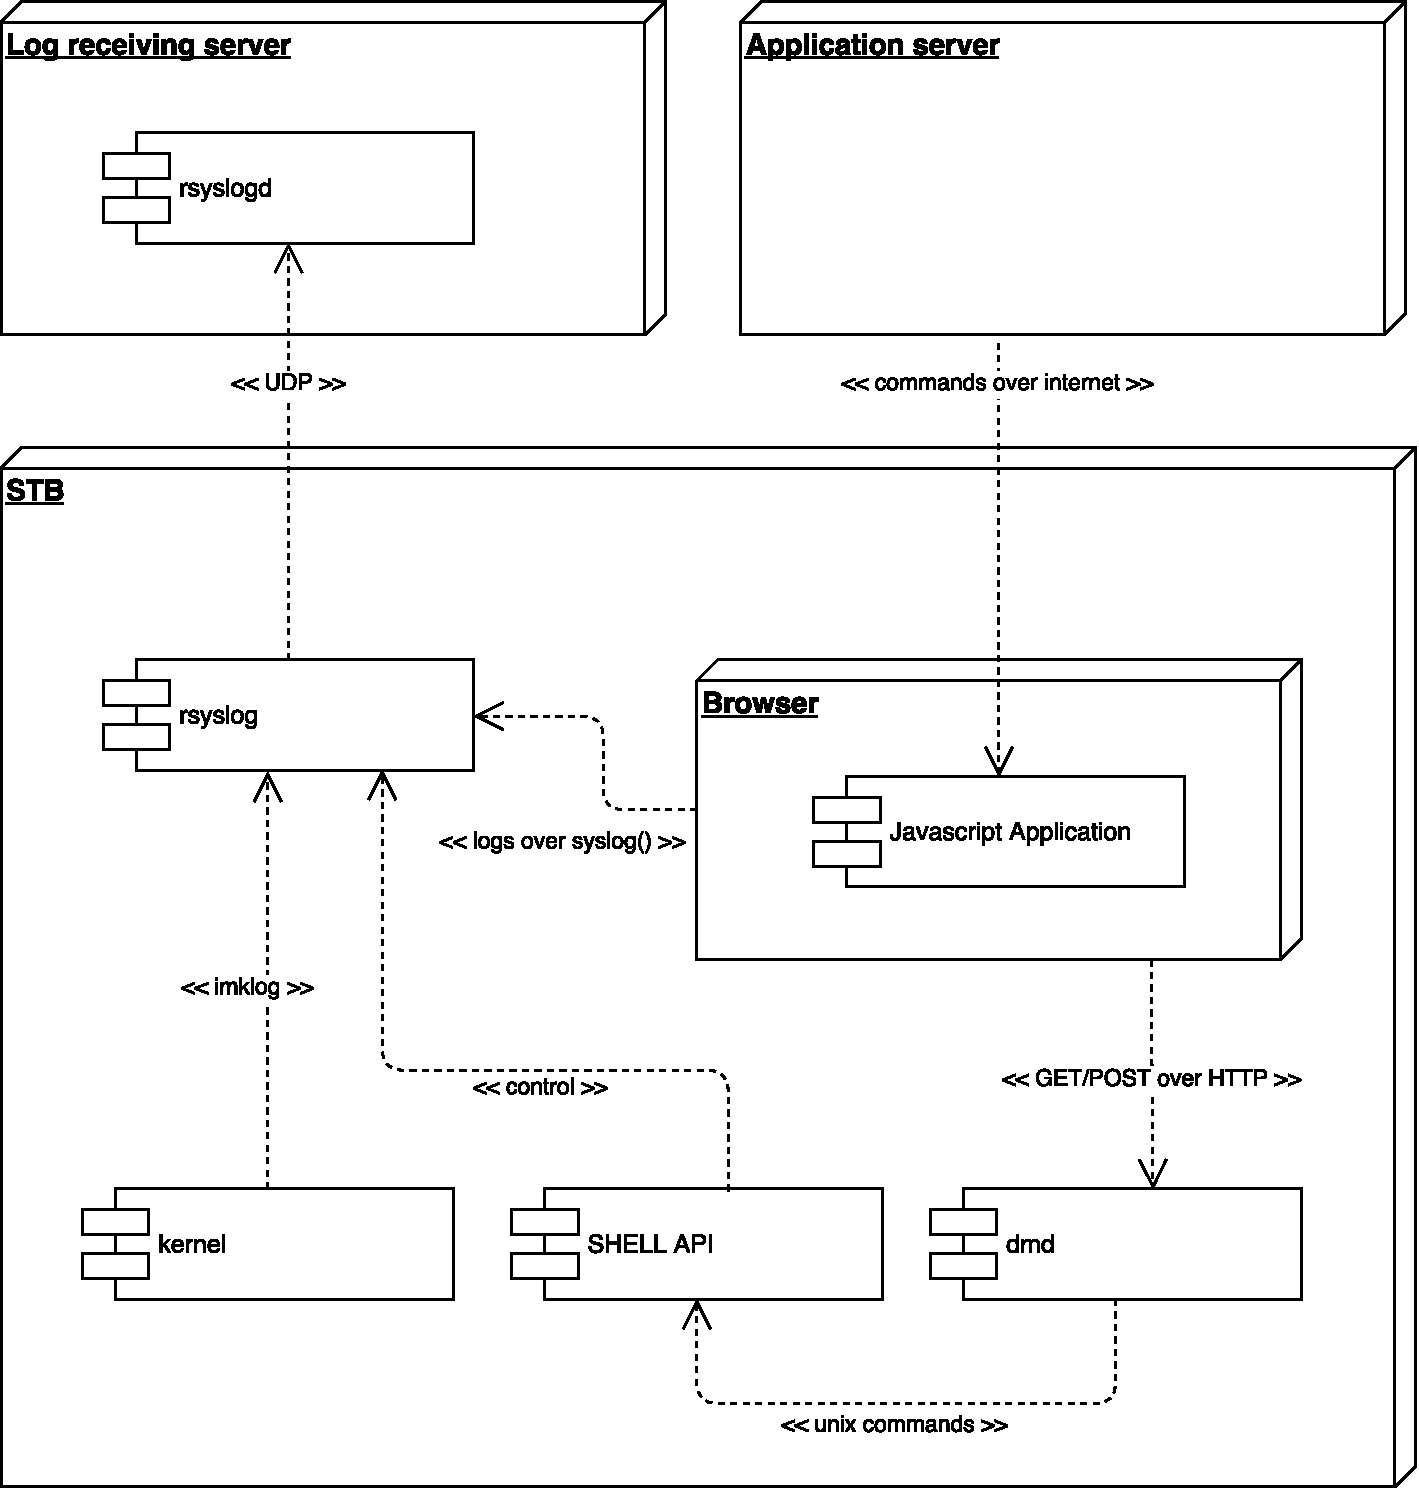
\includegraphics[scale=0.5]{images/diagram-noveho-reseni}
	\caption[Diagram nového řešení]{Diagram nového řešení}
\end{figure}

V oddílu 3.2.1 bylo rozhodnuto o nahrazení logovacího démona Syslogd modernějším Rsyslogem. Ten bude navíc doplněn o API, jež bude umožňovat vzdálenou změnu jeho konfigurace. Komunikace jednotlivých komponent v novém řešení je pro lepší představu znázorněna na obr. 3.2. Je možné si povšimnout, že API bude voláno skrze démona Dmd, jak již bylo nastíněno v oddílu 3.1.2.2.

\chapter{Návrh a realizace}
V úvodu kapitoly je předveden buildovací systém a způsob instalace aplikací pro STB.
Následuje obsáhlý popis Rsyslogu a jeho funkcí včetně ukázek jeho konfigurace.
Dále je popsán vývoj modulů pro Rsyslog, a jsou představeny dva vlastní, naprogramované.
Kapitolu zakončuje návrh API pro vzdálenou konfiguraci Rsyslogu a popis jeho implementace.

\section{Sestavení a instalace Rsyslogu na STB}
Rsyslog není součástí SDK, a tak jej bylo nutné a všechny knihovny na kterých závisí (zlib, libestr, libee, liblogging a libfastjson) zkompilovat, a posléze nainstalovat na STB. K tomu byl použit systém Gu.

\subsection{Buildovací systém Gu}
Gu je buildovací systém pro linuxová embedded zařízení, který si klade za cíl zjednodušit a urychlit buildovací proces. Gu využívá balíčkovací systém pacman (převzatý z Arch Linuxu) a nástroj scratchbox2, sloužící k zjednodušení cross-kompilace. Tyto 2 nástroje jsou skryty v konzolovém přikazu \uv{gu}, kterým se celé Gu ovládá.

\subsection{PKGBUILD}
Jedná se o shellový skript obsahující informace potřebné pro sestavení jednotlivých aplikací systémem Gu. Jeho syntaxe je podrobně popsána v oddílu 4.1.3.
\clearpage 

\subsection{Sestavení a instalace aplikací}
Jako ukázka je níže zobrazen obsah souboru PKGBUILD pro sestavení a instalaci Rsyslogu. V podobném duchu jsou napsány i skripty pro ostatní aplikace a knihovny.
\begin{lstlisting}[style=PKGBuildStyle]
pkgname=rsyslog
pkgver=8.16.0-nangu-0.3
arch=('armv7h' 'armv7sp')
depends=('zlib' 'libestr' 'libee' 'liblogging' 'libfastjson')
source=${pkgname}-${pkgver}.tar.gz
md5sums=('SKIP')

build() {
	cd ${pkgname}
	PKG_CONFIG_PATH=/mnt/hdd_1/lib/pkgconfig
	autoreconf -fvi
	./configure --prefix=/mnt/hdd_1 \
	--disable-uuid --enable-mmsequence \
	--enable-mmsevrewrite --enable-mmdelstr
	make V=1
}

package() {
	cd ${pkgname}
	make install DESTDIR=${pkgdir}
}
\end{lstlisting}

\begin{description}
  \setlength\itemsep{-1ex}
  \item [pkgname:] Název balíčku (měl by se shodovat s názvem zdrojového archivu aplikace).
  \item [pkgver:] Verze balíčku (měla by se shodovat s verzí sestavované aplikace).
  \item [arch:] Pole specifikující architektury cílových systémů.
  \item [depends:] Pole názvů balíčků, které musí být nainstalovány před spuštěním tohoto softwaru.
  \item [source:] Seznam souborů nutných pro sestavení balíčku. Soboury mohou odkazovat na lokální úložiště nebo na vzdálený server (v tom případě se skript postará o jejich stažení). Komprimované soubory skript automaticky rozbalý.
  \item [md5sum:] Pole kontrolních součtů pro každý specifikovaný \uv{source}.
  \item [build():] Nepovinná funkce obsahující příkazy vedoucí ke konfiguraci a sestavení aplikace.
  \item [package():] Povinná funkce instalující soubory. Funkce je spouštěna až po exekuci ostatních nepovinných funkcí.
  \item [pkgdir:] Proměnná obsahující umístění kořenového adresáře instalované aplikace.
\end{description}

Po vstoupení do adresáře obsahujícího zdrojové kódy aplikace a skript PKGBUILD, stačí zadat příkaz \uv{gu build}, čímž se uvede do chodu celý skript. Nejdříve se inicializují proměnné, posléze se vykoná funkce build() a nakonec package(), čímž (pokud nedojde k žádné chybě) vznikne v umístění \uv{pkdir} balíček s přeloženou aplikací.
Příkazem \uv{gu install <název-vzniklého-balíčku.tar.xz>} se balíček nainstaluje do SDK.

\section{Konfigurace Rsyslogu}
Rsyslog se řídí pravidly specifikovanými v konfiguračním souboru rsyslog.conf. Zapnutím tzv. compatibility módu~\cite{Rsyslog-comp-mode} je umožněna podpora syntaxe známá z dříve na Linuxu hojně užívaného démona Sysklogd. Níže je uveden příklad konfiguračního souboru syslog.conf~\cite{Syslog-conf} pro Sysklogd. Na levo je možno specifikovat kritéria pro filtraci zpráv podle jejich severity a facility. Na pravo je pak definováno cílové umístění zpráv.

\begin{lstlisting}[style=AshStyle]
*.=crit;kern.none            /var/adm/critical
kern.*                       /var/adm/kernel
kern.crit                    @finlandia
kern.crit                    /dev/console
kern.info;kern.!err          /var/adm/kernel-info
\end{lstlisting}

Díky této podpoře je možno velice snadno migrovat z démona Sysklogd na Rsyslog.
Ovšem pro využití i jiných než základních funkcí Rsyslogu je nutno k nakonfigurování pravidel použít syntaxi jazyku Rainerscript, který je z toho důvodu v této práci použit.

\subsection{RainerScript}
RainerScript~\cite{RainerScript} je skriptovací jazyk navržený ke správě síťových událostí a nebo ke konfiguraci libovolného softwaru, ačkoli v době psaní této práce byl reálně pužíván pouze v Rsyslogu.
Jedná se o netypový jazyk s podporou regulárních výrazů~\cite{RainerScriptPropertyReplacer}. Podrobnosti jsou k nalezení v dokumentu s formální definicí jazyka~\cite{RainerScriptFormalDefinition}.

\subsection{rsyslog.conf}
V tomto oddílu je uvedena ukázka konfiguračního souboru napsaného jazykem RainerScript, kde jsou předvedeny základní konstrukce používané při jeho tvorbě. Tato ukázka by měla primárně sloužit zadvateli pro porozumění konfiguračního souboru a jako možný návod pro budoucí úpravy.

\begin{lstlisting}[style=RainerScriptSimpleStyle]
module(load="NazevModulu")
\end{lstlisting}
Na začátku souboru je možné načíst různé moduly, poskytující doplňující funkce. Příkladem může být modul imklog, čtoucí zprávy z kernelu, nebo modul omfwd, umoňující posílat zprávy skrze protokoly UDP nebo TCP. Je nutno poznamenat, že některé moduly nejsou ve výchozím nastavení kompilovány spolu s Rsyslogem, a je proto nutno přidat příkazu compile parametr $-$$-$enable$-$<název\_modulu>.

\begin{lstlisting}[style=RainerScriptSimpleStyle]
set $!Promenna="hodnota";
unset $!Promenna;
\end{lstlisting}
Pomocí klíčovích slov set a unset je možné deklarovat a rušit proměnné. Ty začínají znaky \$! a příkaz je nutno ukončit středníkem.

\begin{lstlisting}[style=RainerScriptSimpleStyle]
template(name="template-name" type="string" string="<%pri%>%TIMESTAMP:::date-rfc3164% %$!macaddr% %syslogtag% id=%$!counter%%msg%\n"
	)
\end{lstlisting}
Šablony definují podobu zpráv. Do proměnné string lze vložit libovolné konstantní textové řetězce a dále proměnné, jež se vkládají mezi dvojici znaků procento. Použity mohou být vlastní deklarované proměnné nebo tzv. replacement proměnné, které jsou definovány dokumentací RainerScriptu. Příkladem replacement proměnné může být \uv{app-name}, obsahující název komponenty, jež vygenerovala zprávu nebo \uv{msg}, obsahující text zprávy. 

\begin{lstlisting}[style=RainerScriptSimpleStyle]
action(template="template-name" type="omfwd" Target="192.168.1.10" Port="5514" Protocol="udp" )
\end{lstlisting}

Pomocí akcí se volají jednotlivé moduly. Ty mohou mít různé parametry, které upravují jejich chování. V ukázce výše je volán modul Omfwd, sloužící k posílání zpráv skrze protokoly UDP nebo TCP. Parametry specifikují konkrétní IP a port sítě, typ protokolu a název použité šablony.

\begin{lstlisting}[style=RainerScriptSimpleStyle]
if $programname == 'solid' and $syslogseverity > 5
then {
	#some action
	stop
}
\end{lstlisting}
	
RainerScript podporuje podmíněný příkaz \uv{if}, jež má podobnou syntaxi jako je tomu v jazycích C nebo Java.
V podmínce \uv{if} se obvykle volají různé akce.

Jednořádkové komentáře začínají za symbolem \uv{\#}.
\\
\\
Nyní po obeznámení se základní syntaxí RainerScriptu, je možno popsat fungování zachytávání jednotlivých zpráv. Ty imaginárně putují odshora dolů skrze kód v souboru rsyslog.conf, kde prochází skrze podmínky a akce (které je eventuelně upravují nebo např. zapisují do souborů), a to až do doby, než narazí na klíčové slovo \uv{stop} nebo na poslední řádek souboru.

\subsubsection*{Rsyslog Queues}
\begin{figure}[ht]
	\centering
	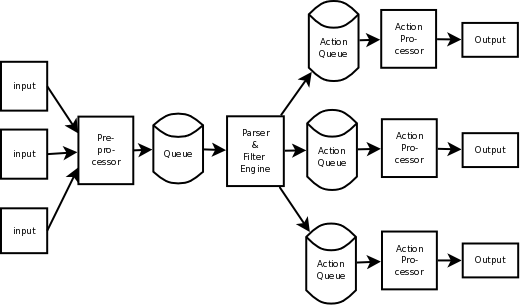
\includegraphics[scale=0.4]{images/rsyslog-queues}
	\caption[Tok zpráv v Rsyslogu]{Tok zpráv v Rsyslogu~\cite{RsyslogQueues}}
\end{figure}

Princip fungování front v Rsyslogu je znázorněn na obrázku 4.1. Zprávy (ať už lokální nebo pocházející ze vzdáleného zdroje) vstupují do Rsyslogu  na obrázku zleva, kde jsou předzpracovány a putují do Main Queue. V dalším kroku jsou zprávy tříděny podle pravidel specifikovaných v rsyslog.conf, a posléze putují do jednotlivých Action Queues. Následně proběhne finální zpracování zpráv a opouštějí Rsyslog skrze výstupní modul, ať už zápisem do lokálního souboru, nebo např. předáním jinému procesu.

Všechny zprávy tedy projdou nejprve skrze Main Queue, a poté skrze libovolný počet Action Queues. Je nutno zmínit, že každá akce obsahuje vlastní frontu, ve které zprávy čekají na zpracování. V případě, že v akci není žádná fronta žádoucí, stačí nastavit typ fronty jako Direct mode.

Existují totiž čtyři módy front. Speciálním (a výchozím) je Direct mode. Direct Queues ve skutečnosti nejsou frontami. Neobsahují totiž žádný buffer a zprávy rovnou přeposílají dál. Vhodné jsou například při zápisu logů do souboru na lokální úložiště.

Druhým typem jsou In-Memory Queues, které udržují zprávy v bufferu v operační paměti. Výhodou je vysoká rychlost a nevýhodou zase hrozba ztráty dat, v případě neočekávaného pádu systému.
In-Memory fronty mohou být implementovány buď formou spojového seznamu (LinkedList Queue), a nebo za použití pole ukazatelů na zprávy (FixedArray) s předem pevně určeným počtem prvků pole. FixedArray mode je nejrychlejší ze všech módů a je vhodný pro případy, kdy se očekává pouze malý počet zpráv ve frontě. Naproti tomu LinkedList Queue dynamicky alokuje místo v paměti pro každou zprávu a je výhodný například na serverech, kde se očekává velký tok zpráv.

Třetí typ front představují Disk Queues, které jak z názvu vyplývá používají disk jako vyrovnávací paměť. Využití najdou v případech, kdy je vyžadována vysoká soplehlivost. Jejich nevýhodou je pomalost limitovaná rychlostí perzistentních úložišť.

Disk-Assisted Memory Queues fungují stejně jako In-Memory Queues, a navíc v případě potřeby dokáží obsah fronty nebo její část přesunout na disk. Používají chytrý algoritmus, který při malém vytížení vůbec nepoužívá Disk Queues. Až v případě vyčerpání kapacity In-Memory fronty se algoritmus postará o přesun části zpráv do diskové fronty.

\subsubsection*{Rate-limiting za použití Rsyslog Queues}
Původní řešení trápil neduh, kdy k vyprázdnění bufferu docházelo až s nově příchozí zprávou, což mělo za následek, že v případě zaplněného bufferu a následující delší odmlky nově příchozích zpráv, mohlo dojít k velkému zpoždení odeslání zpráv v ten moment uložených v bufferu. Tento problém se nasazením Rsyslogu a použitím jeho sofistikovaných front vyřeší.
V tomto oddílu je popsána implementace fronty, která má za cíl škrtit tok odchozích zpráv podle stejných kritérií, jako tomu bylo v původním řešení.

Původní řešení bylo postavené na démonu BusyBox Syslogd, doplněné o vlastní implementaci rate-limitingu zpráv, a fungovalo následovně. Všechny příchozí zprávy putovaly do fronty o fixní velikosti 128 kB. V případě, kdy tok odchozích zpráv překročil 150 kbit/s nebo počet zpráv ve frontě přesáhl 800, byly nově příchozí zprávy zahozeny.

Rsyslog přímo neumožňuje nastavení maximálního toku sítě, avšak poskytuje možnost nastavit pro frontu tyto parametry:
\begin{description}
  \setlength\itemsep{-1ex}
  \item [Queue.Size:] Maximální počet zpráv ve frontě.
  \item [Queue.Dequeuebatchsize:] Maximální počet zpráv vystupujících z fronty v jedné dávce.
  \item [Queue.Dequeueslowdown:] Zpoždění (v $\mu$s) mezi odesíláním dávek zpráv.
\end{description}

Queue.Size je nově nastaven stejně na 800 zpráv.

Parametru Dequeuebatchsize byla přidělena hodnota 10. Z měření totiž bylo zjištěno, že průměrná velikost UDP paketu se zprávou z STB má okolo 150~bytů. MTU UDP paketu je 1500~B. Deset 150-ti bytových paketů se zprávami v součtu odpovídá velikosti jednoho paketu běžně putujícího po síti, a ty tak zaručeně nezpůsobí přetížení linky, způsobené vlivem moc velkého objemu dat naráz.
Dále je hodnota okolo deseti výhodná z důvodu, že příliš malé Dequeuebatchsize vytěžuje CPU kvůli nutnosti častého vyprazdňování fronty. Naopak vysoké hodnoty parametru Dequeuebatchsize (v řádu stovek) způsobují nežádoucí, nárazové a velké objemy zpráv na lince. Deset tedy bylo zvoleno za kompromis.
  
Nyní je třeba zjistit, jakou hodnotu nastavit parametru Dequeueslowdown. Pomocí níže zobrazených vzroců bylo spočítáno požadované zpoždění v mikrosekundách, aby zátěž linky nepřekročila 150 kbit/s.

\begin{description}
	\item $počet~zpráv=\frac{šířka~pásma}{velikost~paketu}=\frac{150~*~1~000~[b]}{8~*~150~[b]}=125$
	\item $slowdown=\frac{1~sekunda}{počet~zpráv}=\frac{1~000~000}{125}*batchsize~=~8~000~*~10~=~80~000~[\mu$$s]$
\end{description}
Ještě zbývá zvolit typ fronty, kde kvůli důrazu na nízké využití zdrojů, byla zvolena implementace používající fixní pole ukazatelů na zprávy.
Výsledný kód pro akci s In-Memory frontou s nastaveným rate-limitingem vypadá následovně:
\begin{lstlisting}[style=RainerScriptSimpleStyle]
action(Type="omfwd" Target="192.168.1.10" port="5514" Queue.Size="800" Queue.Dequeueslowdown="80000" Queue.Dequeuebatchsize="10" Queue.Type="FixedArray" )
\end{lstlisting}

\subsection{Razítkování zpráv}
Požadavkem zadavatele bylo značit všechny zprávy vzestupnou řadou čísel, kvůli rozpoznání případného výpadku některé ze zpráv.
K tomu byl použit modul mmsequence~\cite{RsyslogMmsequence}, který byl nastaven jako je ukázáno v kódu níže.
\begin{lstlisting}[style=RainerScriptSimpleStyle]
module(load="mmsequence")
action(	type="mmsequence"
		from="1"
		to="1048576" # 2^20
		var="$!counter" )
\end{lstlisting}
Proměnná \uv{\$!counter} začíná na čísle \uv{1}, a s každou další příchozí zprávou se zvýší o \uv{1}, dokud nenarazí na maximální hodnotu specifikovanou parametrem \uv{to}, kdy je číslo vyresetováno na původní hodnotu \uv{from}.
Tato proměnná je použita v šablonách, a je tak připojena k tělu každé zprávy.

\subsection{Formát logů}
Požadavkem zadavatele je, aby zprávy měly identický formát, jako tomu bylo u původního řešení. Důvodem je nutnost zachování kompatibility se vzdáleným serverem sbírajícím zprávy ze STB, který vyžaduje pevně daný formát.
\\
\\
Vzor zprávy:
\begin{lstlisting}[style=RainerScriptSimpleStyle]
May  1 19:04:54 cc-b8-f1-04-17-89 solid: id=8853 Player Time [00:06:56.96]
\end{lstlisting}
Formát:
\begin{lstlisting}[style=RainerScriptSimpleStyle]
<PRI><RFC3164 date> <STB mac address> <component>: <id=NUM>  <message>
\end{lstlisting}
Požadovaného formátu bylo dosaženo vhodným nastavením šablony, které je zobrazeno v oddíle 4.2.2.
\clearpage

\section{Moduly pro Rsyslog}
Rsyslog poskytuje podporu tzv. modulů, které mohou zásadně rozšiřovat jeho rozsah funkcí. Tyto moduly jsou obvykle napsány v jednom C souboru. Pro jejich zprovoznění je třeba náležitě upravit Makefile a zkompilovat Rsyslog se zapnutou podporou pro ně.

Moduly se dělí na šest základních kategorií, zde jsou zmíněny tři nejpoužívanější:

\begin{description}
  \item [Output Modules:] Výstupní moduly umožňují posílat zprávy na různé cíle. Je tak možno implementovat například modul, který dokáže odesílat zprávy do nějaké exotické databáze, kterou Rsyslog v základu nezná. Příkladem výstupního modulu je Ommail sloužící k posílání zpráv skrze mail.
  \item [Input Modules:] Vstupní moduly, jak název napovídá, umožňují přijímat zprávy z různých zdrojů. Hojně používaný je Imklog, sbírající zprávy z linuxového jádra nebo Imudp, přijímající zprávy skrze protokol UDP.
  \item [Message Modification Modules:] Moduly, které modifikují obsah zprávy. Příkladem je v této práci použitý modul Mmsequence, který generuje číselné řady.
\end{description}

V této práci byly naprogramovány dva moduly, oba z kategorie Message Modification Modules. V následujícím textu je popsán jejich účel a způsob použití. Implementace není v práci uvedena, protože se většina kódu skládá z volání API Rsyslogu, a navíc zdrojový kód každého z modulů obsahuje stovky řádků.

\subsection{Modul mmdelstr}
Tento modul slouží ke smazání zadaného podřetězce z těla zprávy.
\\
\\
Použití:
\begin{lstlisting}[style=RainerScriptSimpleStyle]
module(load="mmdelstr") 
action(type="mmdelstr" stringtobedeleted="Some string")
\end{lstlisting}

Modul má pouze jeden parametr (stringtobedeleted), kterým se specifikuje podřetězec, který má být smazán. V případě neexistence takového podřetězce zůstává zpráva netknutá. V případě výskytu vícero takových podřetězců je smazán pouze první.

\subsection{Modul mmsevrewrite}
Mmsevrewrite dokáže měnit severitu zpráv. Rsyslog v základu funkci s takovou schopností nenabízí, jelikož se jedná o neobvyklý požadavek. Modul je v této práci použit  pro konverzi zpráv pocházejících z aplikace používající s Rsyslogem jinak nekompatibilní množinu severit.
\\
\\
Použití:
\begin{lstlisting}[style=RainerScriptSimpleStyle]
module(load="mmsevrewrite")
action(type="mmsevrewrite" severity="debug")
\end{lstlisting}

Modul obsahuje pouze jeden parametr \uv{severity}, kterým se určuje nová severita zprávy. V případě zadání neplatné severity Rsyslog zaloguje chybovou hlášku a upravovaná zpráva zůstane v původním stavu.

\subsection{Postprocessing zpráv}
Zadavatel požaduje vytvoření tří ukázkových pravidel pro RainerScript, podle kterých si v budoucnu vytvoří sadu vlastních pravidel.

\subsubsection{Zahazování zpráv podle typu komponenty}
Pravidlo, které rozpozná zprávu (podle typu komponenty, jež ji vygenerovala a obsahu jejího textu) a v případě shody ji zahodí.
\\
\\
Implementace pravidla:
\begin{lstlisting}[style=RainerScriptStyle]
if $programname == 'solid' and \
$msg contains "Player_GetState" then
{	
	stop
}
\end{lstlisting}
Pokud zpráva pochází z komponenty \uv{solid} a obsahuje zmíněný podřetězec, klíčové slovo \uv{stop} okamžitě zahodí v ten moment zpracovávanou zprávu.
\\
\subsubsection{Převod severit}
Některé aplikace běžící na STB používají jinou množinu severit, než s jakými pracuje Rsyslog, a navíc nejsou v hlavičce zprávy, nýbrž v jejím těle.
Zadavatel proto požaduje severity zpráv extrahovat z jejich těl a nastavit je podle tabulky 4.1.

\begin{table}[H]
\centering
	\caption{Převodní tabulka severit}	\begin{tabular}{|l|l|}\hline
		Portal		& Syslog			\tabularnewline \hline \hline
		ERROR		& ERR			\tabularnewline \hline
		WARN		& WARN			\tabularnewline \hline
		INFO		& NOTICE			\tabularnewline \hline
		DEBUG		& INFO			\tabularnewline \hline
		TRACE		& DEBUG			\tabularnewline \hline
	\end{tabular}
\end{table}
Implementace pravidla:
\begin{lstlisting}[style=RainerScriptStyle]
if $msg contains "mTRACE: " then
{
	action(type="mmsevrewrite" severity="debug")
}
else if $msg contains "mDEBUG: " then
{
	action(type="mmsevrewrite" severity="info")
}
\end{lstlisting}
Zprávy obsahující nesprávně nastavené severity je možno opravit podle výše zmíněného pravidla. Bylo totiž vypozorováno, že ony postižené zprávy obsahují podřetězec ve formátu \uv{m<SEVERITY>: }. Stačí pak na danou zprávu zavolat akci mmsevrewrite s parametrem severity vyplněným podle převodní tabulky z obr. 4.1.

\subsubsection{Smazání podřetězce z těla zprávy}
Zprávám pocházejícím z komponenty solid je třeba smazat zadaný podřetězec.
\\
\\
Implementace pravidla:
\begin{lstlisting}[style=RainerScriptStyle]
if $programname == 'solid' and $msg contains
		":[notificationFromPlayer]: INFO: " then
{
	action(type="mmdelstr" \ 
	stringtobedeleted=":[notificationFromPlayer]: INFO: ")
}
\end{lstlisting}


\section{Vzdálená konfigurace}
Požadavkem zadavatele je umožnit změnu nastavení maximální povolené severity jednotlivých komponent. Rsyslog neumožňuje změnu konfiguračního souboru za jeho běhu, a proto je nutno implementovat API, které umožní přenastavení konfiguračního souboru a jeho znovunačtení (restartováním Rsyslogu).
Změny tímto skriptem způsobené musí být zachovány i po restartu STB.

\subsection{Návrh API}
Skript musí umět nastavit konfiguraci souboru rsyslog.conf tak, aby v případě rozpoznání zprávy od určité komponenty spolu s nastavenou severitou vyšší, než je povolená, danou zprávu zahodil. 
Musí tedy umět v daném skriptu nalézt část kódu, kde se zpracovává zadaná komponenta, a tuto část kódu vhodně upravit.

V úvahu připadaly 2 různé přístupy. Je možné při každém zavolání skriptu generovat celý nový konfigurační soubor, a nebo pouze části souboru pomocí skriptu měnit.
Výhodou prvního způsobu je, že nehrozí nechtěné přepsání jiných čásí skriptu, než bylo zamýšleno. Nevýhodou je složitější implementace z důvodu nutnosti pří generování nového skriptu zohledňovat předchozí nastavení skritpu. Tedy by bylo nutné z původního skriptu extrahovat nastavení jednotlivých komponent, a to posléze zkombinovat s novým nastavením.
A proto byl zvolen 2. způsob řešení s tím, že zadavatel bude poučen o nutnosti dodržovat určité zásady při měnění konfiguračního souboru, aby nemohlo dojít k přepsání nesprávných částí souboru.

\subsection{Výběr implementačních nástrojů}
Jazyky jako Perl nebo Python se jeví jako ideální pro napsánání skriptu na zpracování textu. Tyto, ani jiné podobné jazyky ovšem nejsou součástí SDK  a zadavatel si nepřeje jejich instalaci z důvodu omezené paměti a omezeného výkonu embedded zařízení. Proto byl zvolen již na STB přítomný příkazový procesor ASH. Ten sice neposkytuje tak elegantní syntaxi a nenabízí tolik schopností jako moderní Shellové jazyky jako např. BASH, ale i přesto je možné jeho použitím spolu se základními Unixovými nástroji API naprogramovat.

\subsection{Rozhraní skriptu}
První zvažovanou variantou je napsat API ve formě skriptu, který přijímá jednotlivé názvy komponent a jim příslušící maximální povolenou severitu jako parametry.

\begin{lstlisting}[style=RainerScriptSimpleStyle]
set_log_verbosity.sh [component1 severity1] ...
\end{lstlisting}
Druhou možností je skript, který čte seznam jednotlivých komponent a maximálních povolených severit ze souboru, který má následující formát:

\begin{lstlisting}[style=RainerScriptSimpleStyle]
component1  = DEBUG
componentXY = INFO
...
DEFAULT     = INFO
\end{lstlisting}
V implementaci byl nakonec použit první způsob, pro jeho jednoduší obsluhu, a navíc s jeho použitím zadavateli odpadá starost o další konfigurační soubor.

\subsection{Implementace API}
API na vstupu očekává sudý počet parametrů, kde každý sudý parametr je název komponenty a liché parametry slouží pro definování severit pomocí jejich číselných hodnot.
Skript vyhledá v konfiguračním souboru rsyslog.conf řádek s danou komponentou a přenastaví maximální povolenou severitu. Skript kontroluje správnost vstupních parametrů, kvůli zabránení neočekávanému chování programu. Nakonec se restartuje Rsyslog, aby načel novou konfiguraci.


\chapter{Testování}
V této kapitole jsou předvedeny tři typy testů.
Nejprve se sleduje využití linky sítě při simulaci běžného provozu STB. Druhý test ověřuje funkčnost rate-limitingu zpráv. A v posledním testu se zkoumá vytížení prostředků STB za běžných i extrémních podmínek.

Vždy je porovnáváno nové řešení postavené na Rsyslogu oproti původnímu.

\section{Testovací prostředí a nástroje}

\subsection{WireShark}
Tento nástroj slouží jako analyzér síťového provozu. Dokáže v reálném čase zachytávat informace o paketech putujících po síti, a ty následně vyzobrazit v grafu. Všechny grafy z této kapitoly jsou vygenerovány tímto nástrojem.

\subsection{Testovací infrastruktura}
Pro účely testování byla nakonfigurována lokální síť, jakožto simulace reálných serverů provozovatele. Jako server pro zachytávání zpráv z STB byl použit notebook Apple Macbook Pro, na kterém byl nakonfigurován logovací démon Syslog-ng.

\section{Test využití linky za běžného provozu}
 V tomto testu je srovnáváno vytížení linky za použití nového a starého logovacího řešení, při běžném provozu STB. 

\begin{figure}[H]
	\centering
	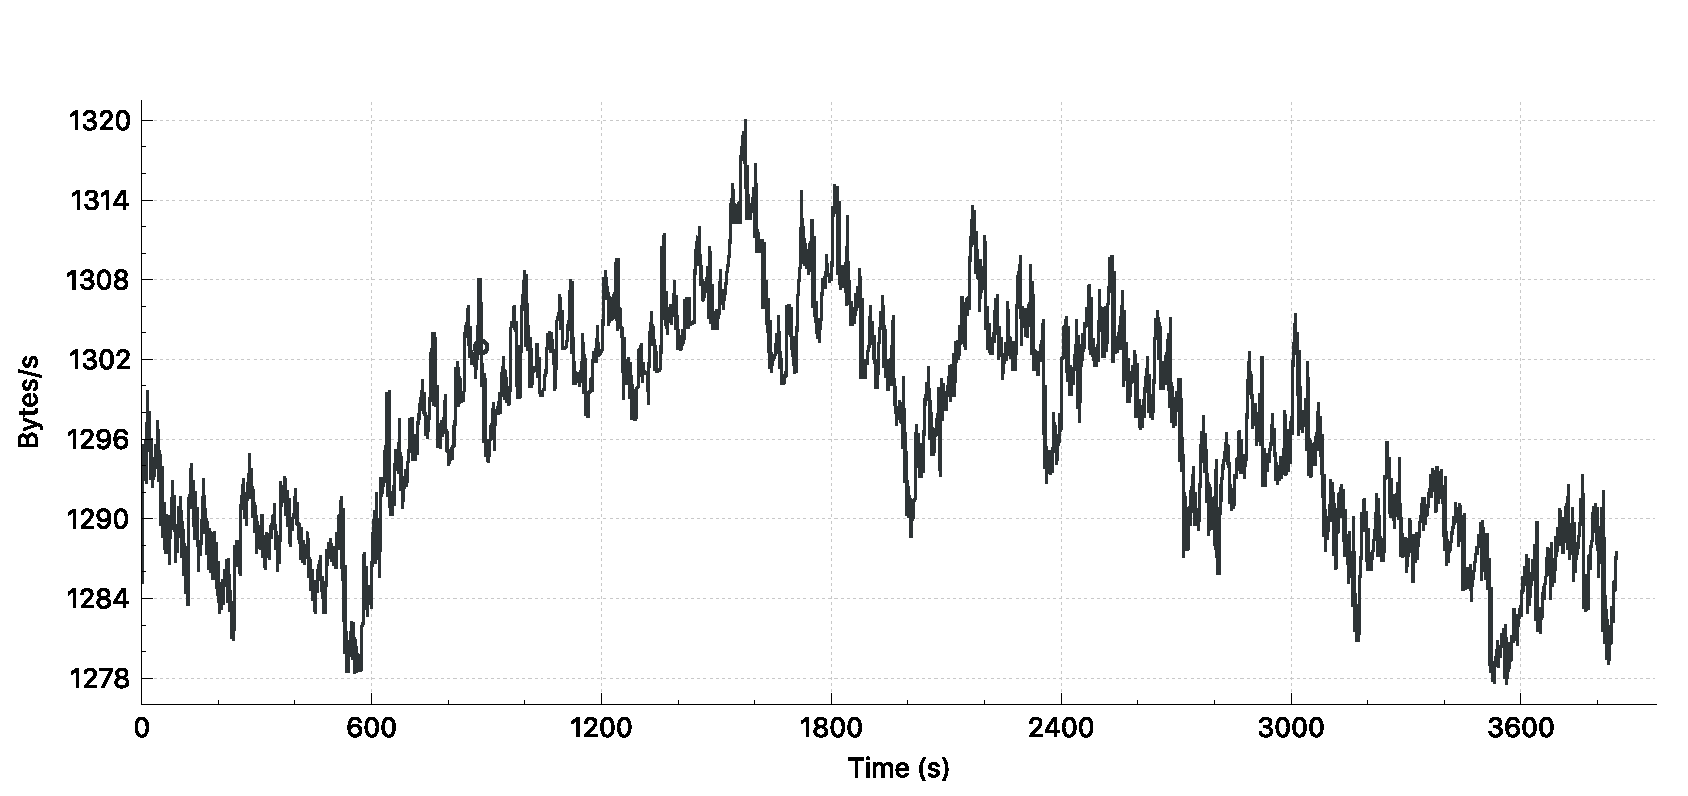
\includegraphics[scale=0.44]{images/test-1h-syslogd-default}
	\caption[Využití linky v původním řešení]{Využití linky v původním řešení}
\end{figure}

\begin{figure}[H]
	\centering
	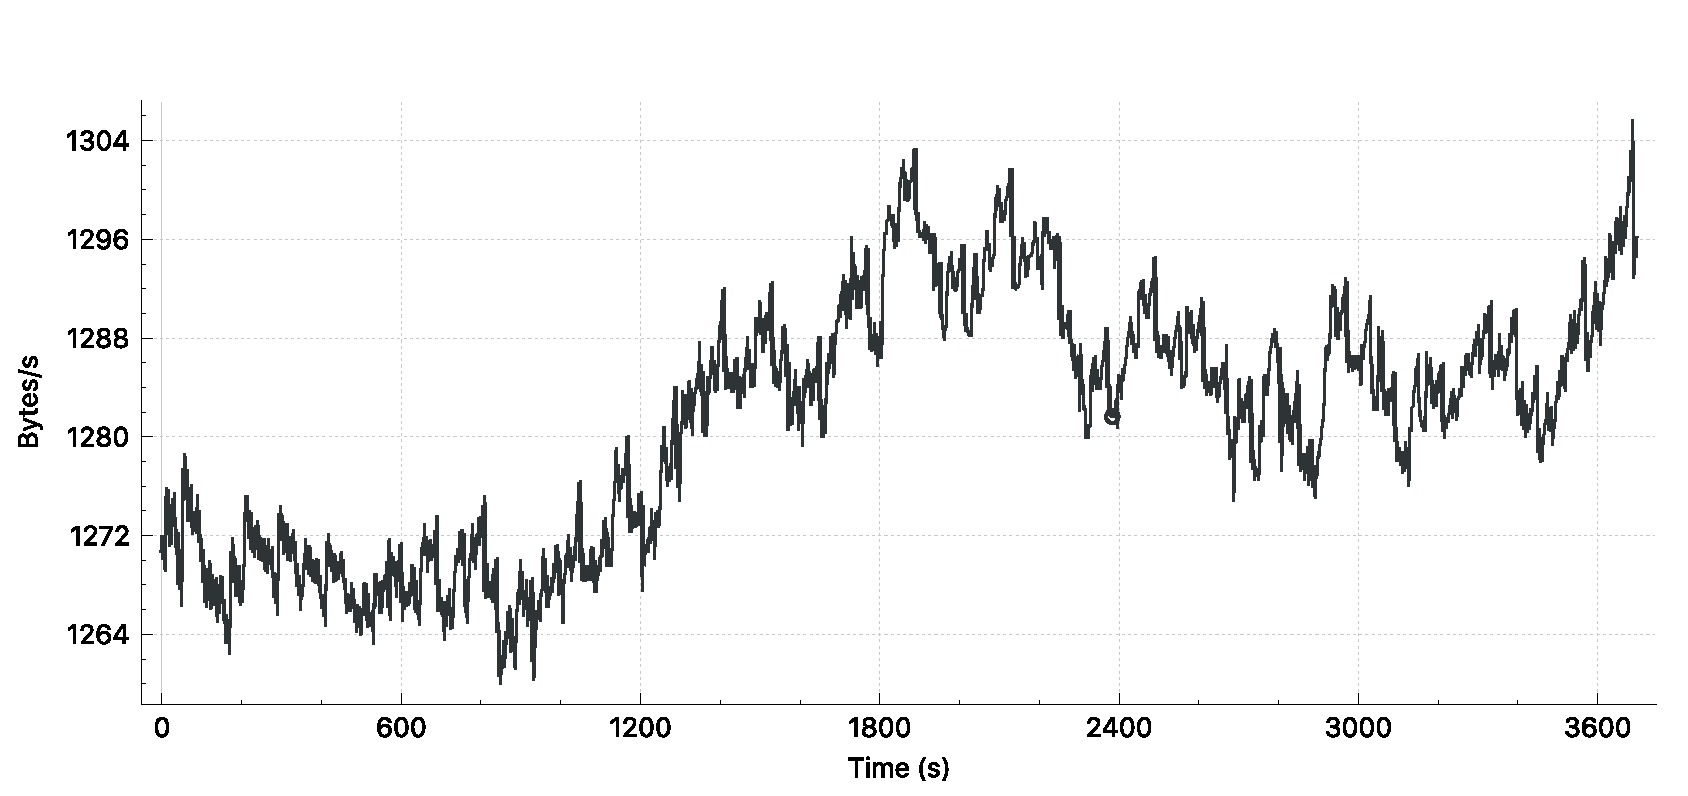
\includegraphics[scale=0.44]{images/test-1h-rsys-default}
	\caption[Využití linky v novém řešení]{Využití linky v novém řešení}
\end{figure}

\begin{figure}[H]
	\centering
	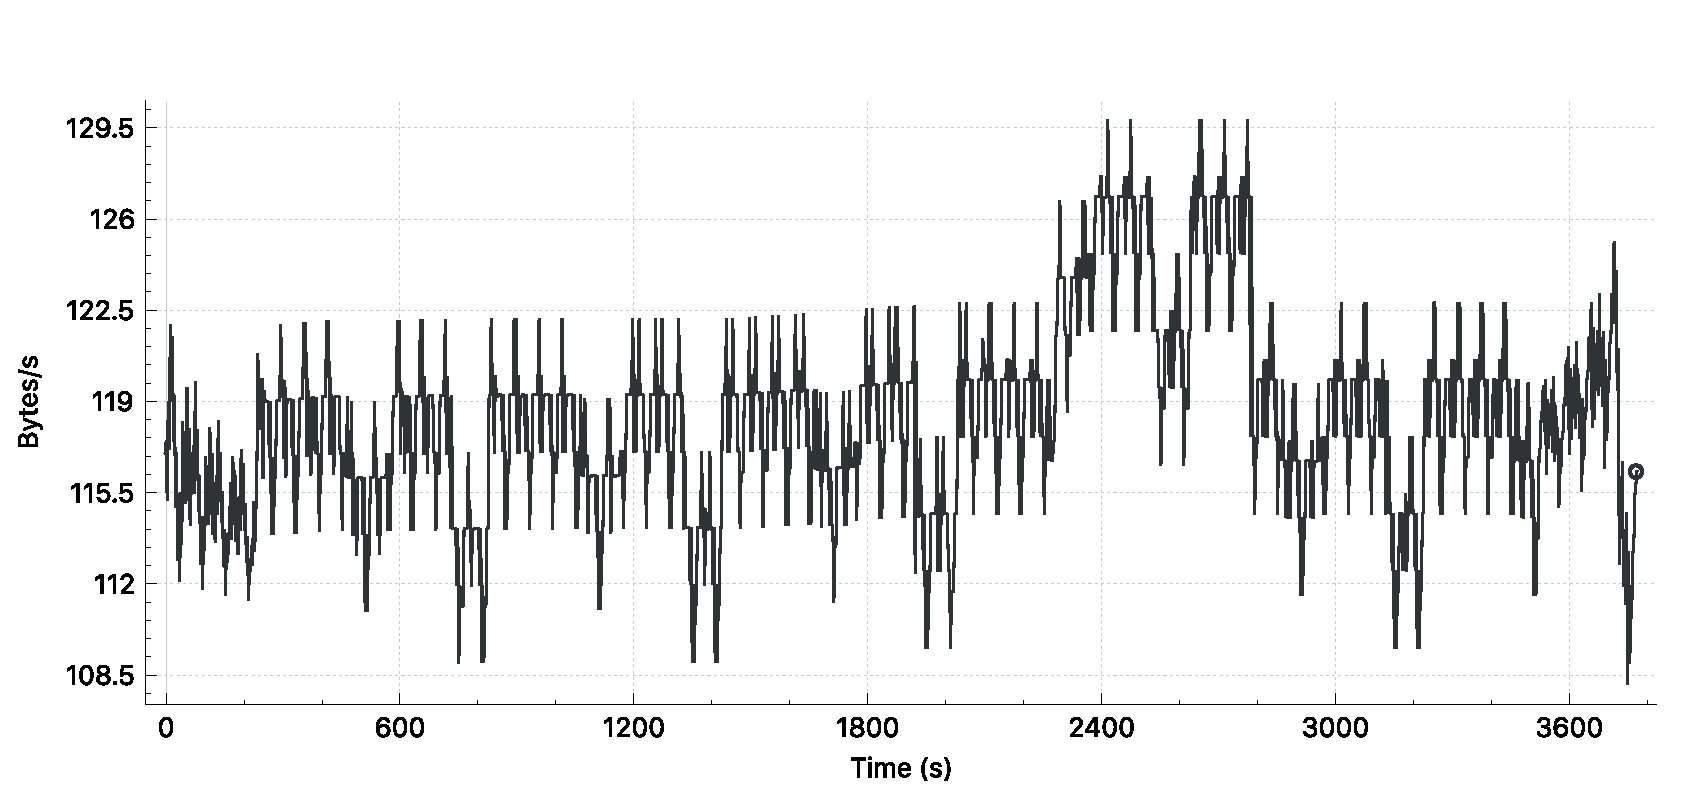
\includegraphics[scale=0.44]{images/test-1h-rsys-solidoff}
	\caption[Využití linky v novém řešení (filtrování zpráv aplikace solid)]{Využití linky v novém řešení (filtrování zpráv aplikace solid)}
\end{figure}

\subsection*{Zhodnocení}
Jak je vidět z prvních dvou grafů (obr. 5.1 a 5.2), nové řešení postavené na démonu Rsyslog přijíma méně logů. Je to způsobeno jeho konfigurací, v níž je nastaveno pravidlo (viz oddíl 4.3.3.1), kterým se zahazují nepotřebné zprávy. Na STB totiž běží aplikace, již zadavatel nemá možnost upravit, která loguje mimo jiné i nepotřebné zprávy. V původním řešením podobné pravidlo nebylo možné jakkoli nastavit.
Dle Wiresharku nové řešení přijímá v průměru 8,6 paketů za sekundu, oproti 9 paketům za sekundu v původním řešení.

Na třetím grafu (obr. 5.3) je pro zajímavost znázorněno využití linky při použití nového řešení, po nastavení filtrace zpráv od komponenty solid.
Účelem bylo demonstrovat, že zadavatel má v novém řešení možnost upravit filtrování zpráv podle různých kritérií, a může tak razantně snížit tok zpráv na síti.

\section{Test rate-limitingu zpráv}
Jak bylo zjištěno v minulém testu, zprávy generované set-top boxem tvoří tok o přibližně deseti tisících bitech za sekundu. Limit toku je nastaven na patnáctinásobek této hodnoty, a tak by se v reálných podmínkách neměl nikdy aktivovat. Nicméně zadavatel rate-limiting požaduje jako pojistku pro případ, kdy by například vlivem chyby některá z komponent začala generovat nepřiměřené množství zpráv, a nedošlo tak k zahlacení ať už sítě na straně uživatele STB nebo serverů provozovatele.

Pro ověření funkčnosti rate-limitingu byl proto sestrojen následující skript.

\subsection{Skript pro otestování rate-limitingu}
Účelem skriptu je generovat takové množství zpráv, aby na síti vznikl tok přesahující 150~000 b za sekundu, a tedy aby logovací démon byl nucen zprávy bufferovat.

Skript je řešen tím způsobem, že je v deseti paralelních instancích zavolán for-cyklus, každý generující po tisíci zprávách.
Zprávy mají konstantní velikost 60 B, což odpovídá délce průměrné zprávy generované set-top boxem.

\begin{lstlisting}[style=AshStyle]
gen_messages() {
	for i in $(seq 1000); do
		logger 	"Lorem ipsum dolor sit amet, consectetuer adipiscing elit."
	done
}

for i in $(seq 10); do
	gen_messages &
done
\end{lstlisting}

\begin{figure}[H]
	\centering
	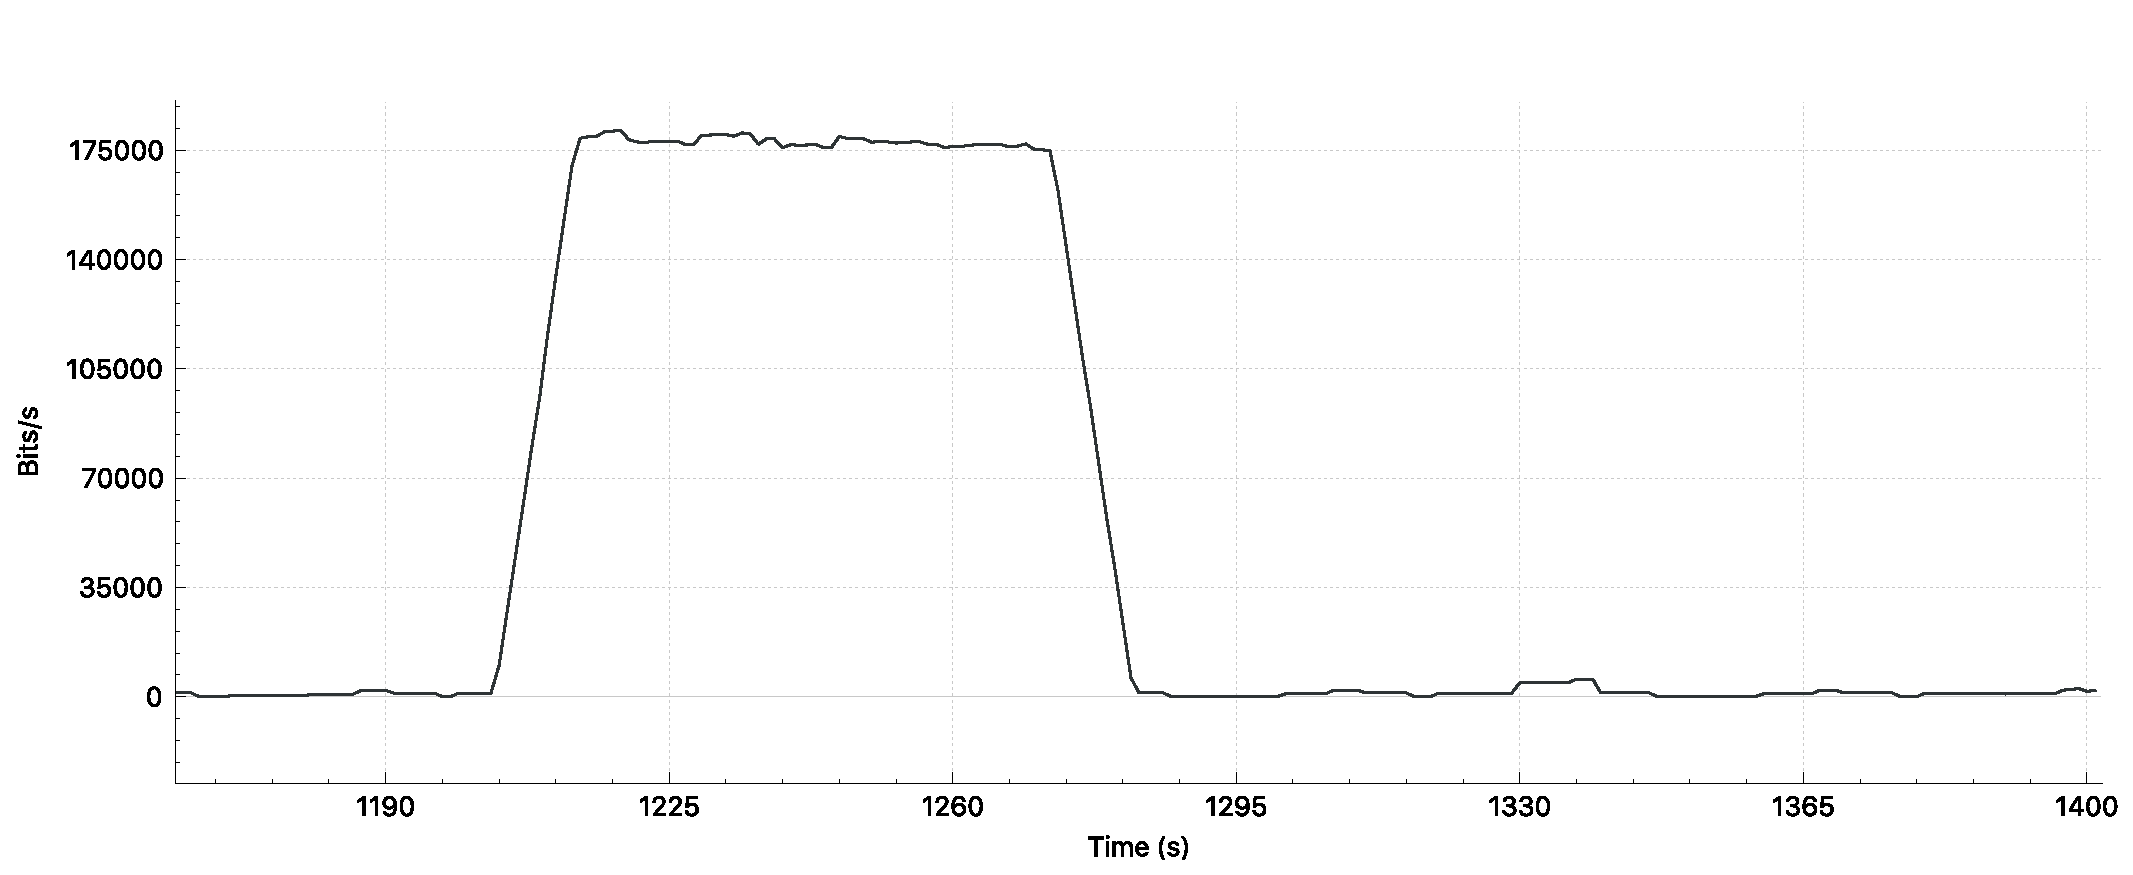
\includegraphics[scale=0.36]{images/test-rateLim-rsyslog-Buff-off}
	\caption[Využití linky při extrémním zatížení bez rate-limitingu]{Využití linky při extrémním zatížení bez rate-limitingu}
\end{figure}
\begin{figure}[H]
	\centering
	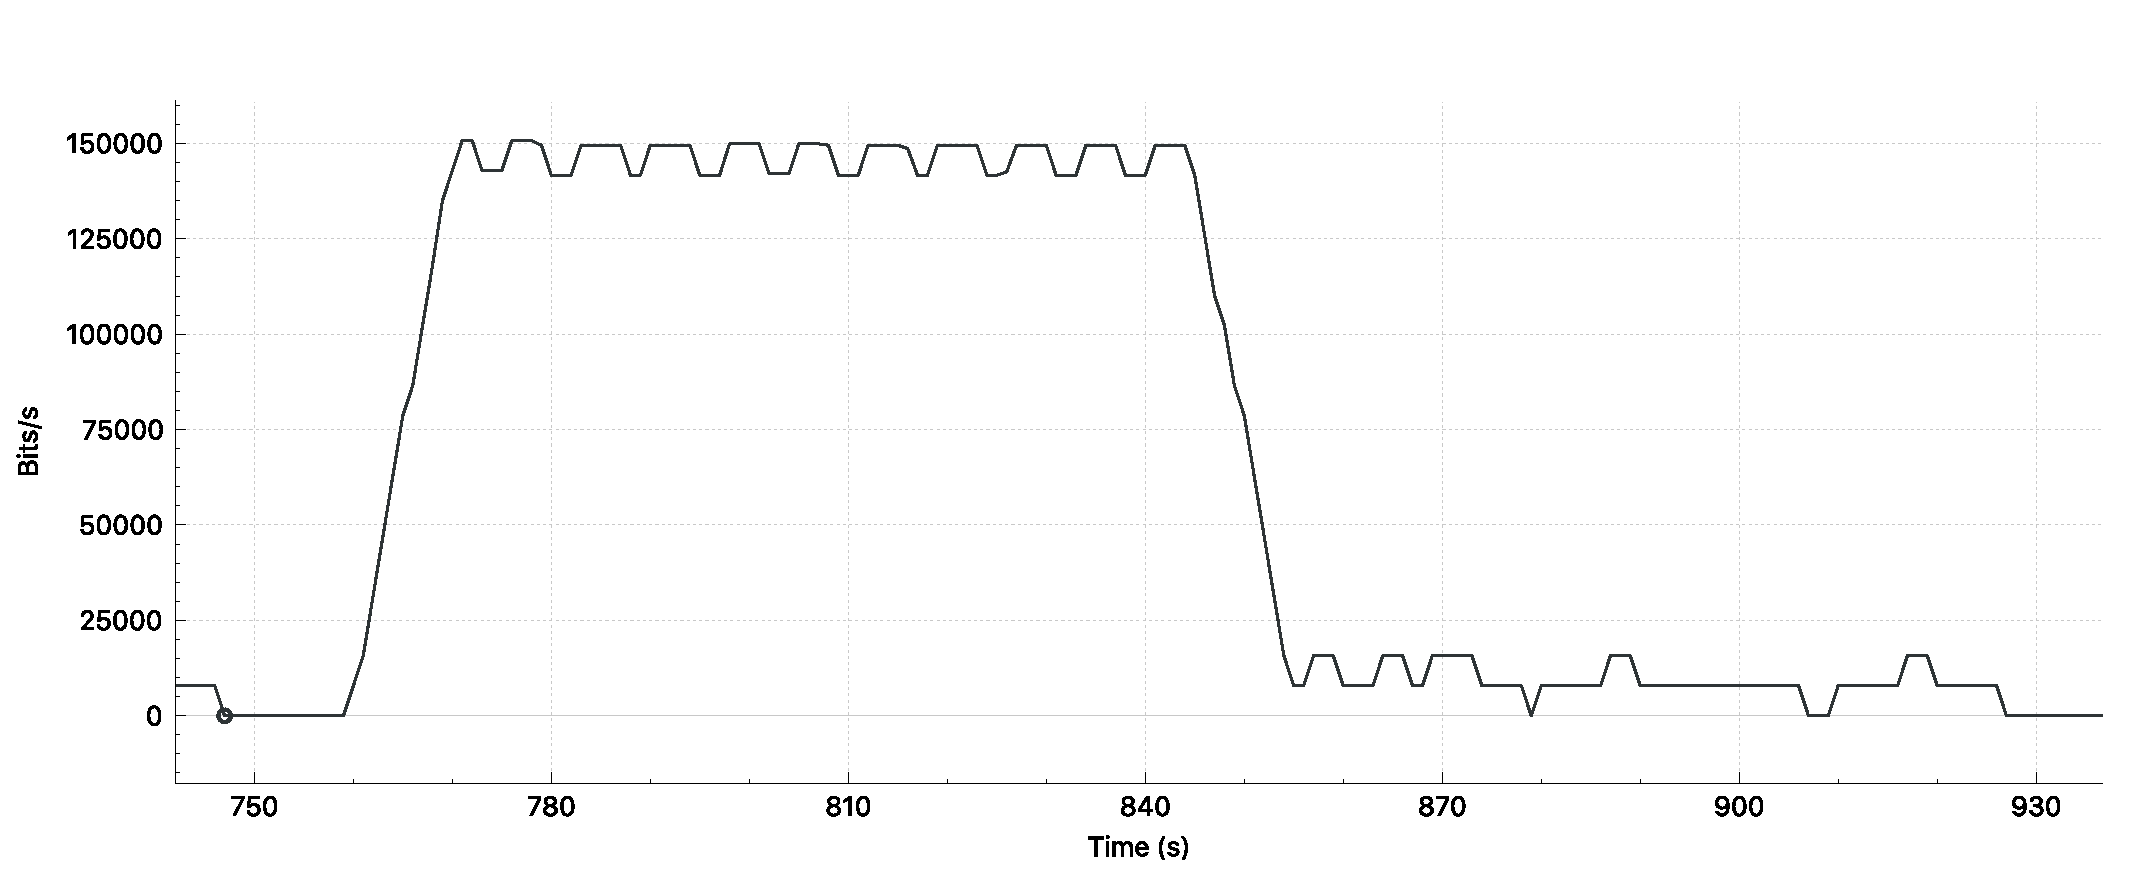
\includegraphics[scale=0.36]{images/test-rateLim-syslogd}
	\caption[Využití linky v původním řešení při extrémním zatížení]{Využití linky v původním řešení při extrémním zatížení}
\end{figure}
\begin{figure}[H]
	\centering
	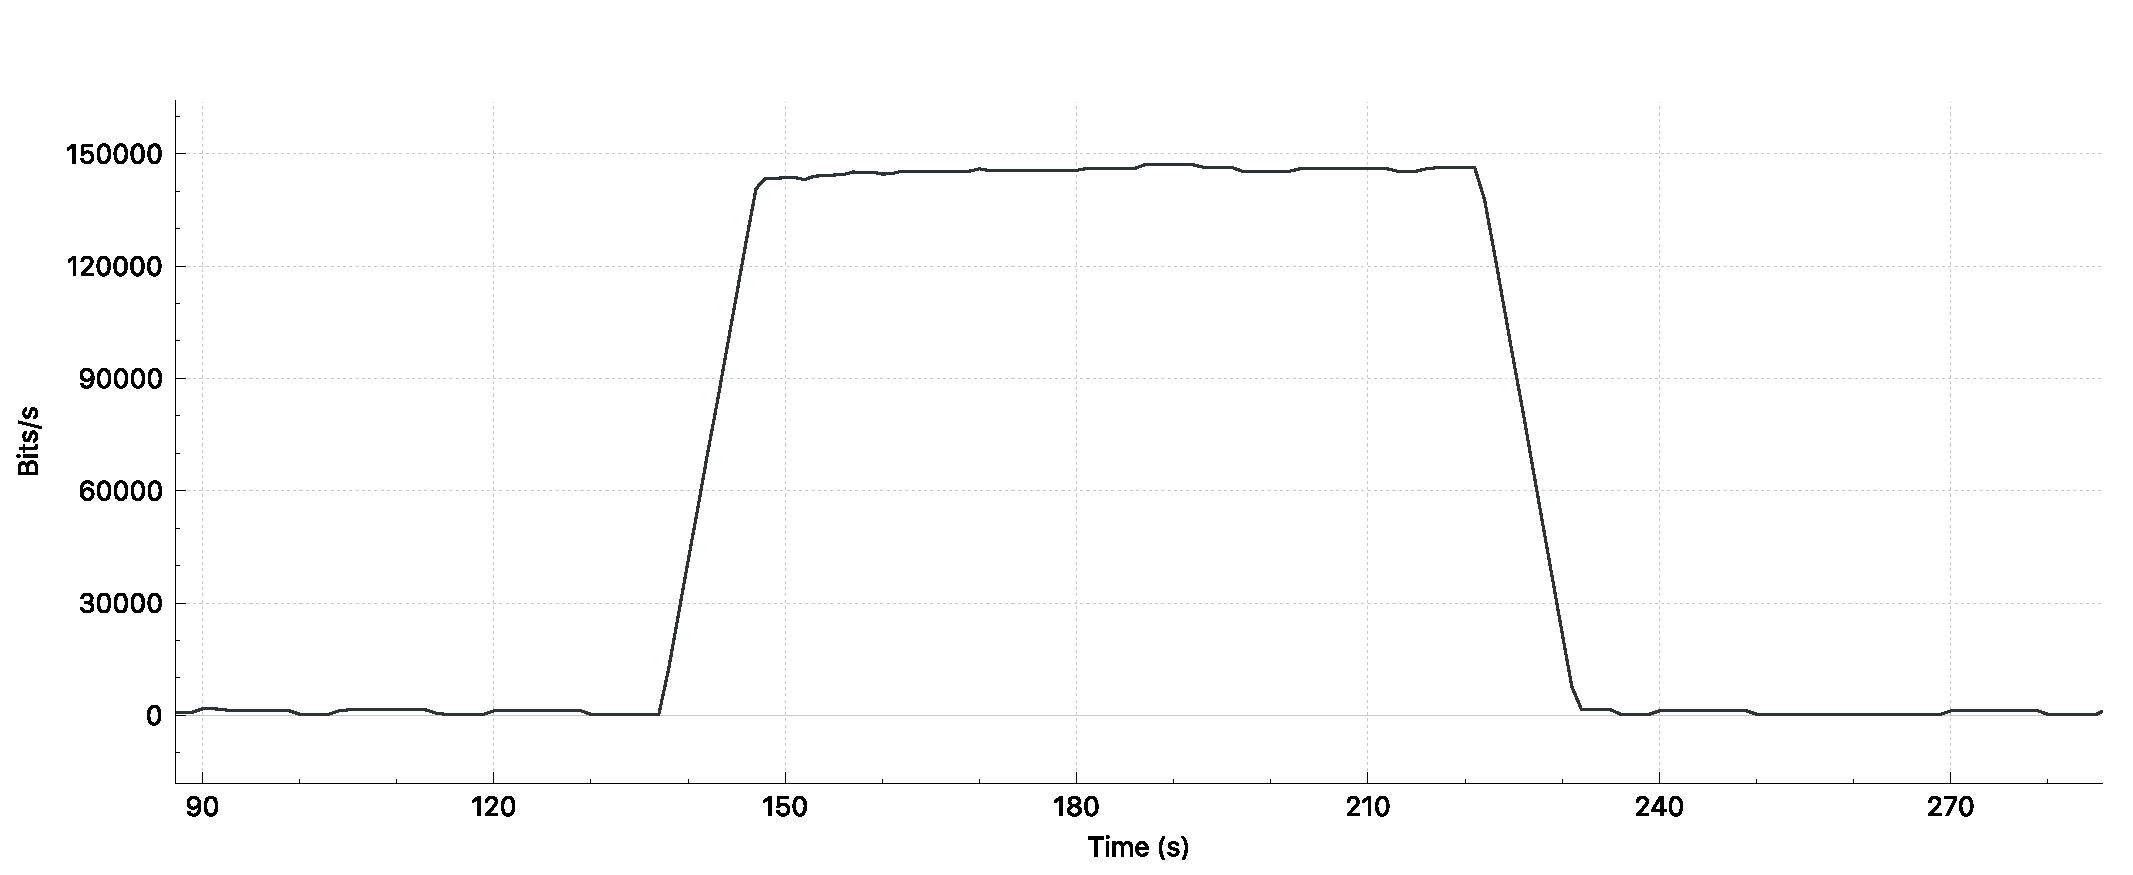
\includegraphics[scale=0.36]{images/test-rateLim-rsyslog}
	\caption[Využití linky v novém řešení při extrémním zatížení]{Využití linky v novém řešení při extrémním zatížení}
\end{figure}

\subsection{Zhodnocení}
První graf (obr. 5.4) znázorňuje kolik bitů textu za sekundu daný skript ve skutečnosti generuje. Graf vznikl použitím Rsyslogu s deaktivovaným Rate-limitingem zpráv.
Zbylé dva grafy (obr. 5.5 a 5.6) pouze demonstrují správnou funkčnost rate-limitingu. Tedy, že tok bitů za sekundu nepřekročí hranici 150~000.

\section{Test vytížení systému}
Protože embedded zařízení neoplývají vysokým výkonem, a ani v této práci použitý STB není vyjímkou, je nutno logovací řešení podrobit testům a zjistit jeho chování pod extrémím zatížením, zda nehrozí jeho přetížení, a z toho vyplývající nestabilita. Dále je otestováno i vytížení systému za běžných podmínek, kde je porovnáno s původním řešením. V testech se zkoumá vytížení CPU a paměťová náročnost.

Před samotným testováním je ale nutno čtenáře seznámit se základními pojmy týkajícími se měření výkonosti CPU v linuxových systémech~\cite{MeasuringPerformance}.

\subsection{Terminologie}

\begin{description}
\setlength\itemsep{-1ex}
	\item [Clock tick:] Clock tick je jednotka pro měření CPU času.
	\item [CLK\_TCK:] Makro (může mít i jiný název jako např. CLOCKS\_PER\_SEC) definující počet clock ticků za sekundu. Na našem STB má hodnotu 100.
	\item [CPU time (CPU čas):] Představuje dobu, kterou procesor strávil vykonáváním procesu vyjádřenou počtem clock ticků nebo v sekundách, získaných vydělením clock ticků hodnotou makra CLK\_TCK.
	\item [User time:] CPU čas strávený vykonáváním procesu v \uv{user režimu}. V tomto řežimu proces nemá oprávnění provádět privilegované operace, které mohou ovlivnit celý systém.
	\item [System time:] CPU čas strávený vykonáváním instrukcí procesu v \uv{kernel režimu}. V tomto řežimu jádro systému provádí privilegované operace vyžádané procesem.
	\item [Real time:] Čas doby běhu procesu v sekundách. Jedná se o absolutní dobu běhu programu, a je v ní tedy i zahrnuta doba, kdy byl proces blokován nebo kdy se dělil o prostředky CPU s jinými procesy.
	\end{description}

\subsection{VFS /proc}
V Linuxových systémech existuje virtuální souborový systém /proc~\cite{procFilesystem}, který v jednotlivých podsložkách a souborech shromažďuje informace o HW systému a procesech v něm běžících.

Informace o stavu procesu shromažďuje soubor /proc/<pid>/stat/ (pid značí číselný identifikátor zkoumaného procesu), který je ve formě textového řetězce obsahujícího informace o procesu. Pro tuto práci důležité informace z tohoto souboru jsou popsány v odstavci níže. Čísla v závorkách představují jejich pozice v řetězci.

\begin{description}
\setlength\itemsep{-1ex}
	\item [utime:] CPU čas strávený vykonáváním procesu v user režimu. (14)
	\item [stime:] CPU čas strávený vykonáváním procesu v kernel režimu. (15)
	\item [cutime:] CPU čas strávený čekáním na potomky procesu v user režimu. (16)
	\item [cstime:] CPU čas strávený čekáním na potomky procesu v kernel režimu. (17)
	\item [starttime:] CPU čas vyjadřující moment startu procesu. (22)
\end{description}

\subsection{Vytížení CPU logovacím démonem při velké zátěží}
V tomto testu je měřeno procentuální vytížení CPU logovacím démonem při extrémních podmínkách. Ty jsou simulovány skriptem z oddílu 5.2.1, který generuje velké množství zpráv, a zahlcuje tak logovacího démona. 

\subsection*{Skript pro získání vytížení CPU}
Skript měří počet clock ticků sledovaného procesu po dobu, kdy je zatížen zpracováním zpráv z paralelně spuštěného skriptu na generování zpráv z oddílu 5.2.1. Poměr takto získanách clock ticků ku celkovému CPU času skriptu genMessages.sh potom představuje procentuální vytížení procesoru daným logovacím démonem.

\begin{lstlisting}[style=AshStyle]
sfile=/proc/$1/stat
if [ ! -r $sfile ];
	then echo "pid $1 not found in /proc"; exit 1;
fi
start=$(cat $sfile| awk '{sum=$14+$15+$16+$17; print sum}')
time ./genMessages.sh 2> timeOut && \
stop=$( cat $sfile| awk '{sum=$14+$15+$16+$17; print sum}')

sysTime=$(cat timeOut | grep sys | awk '{print $3}' | tr -d 's')
userTime=$(cat timeOut | grep user | awk '{print $3}' | tr -d 's')
rm -rf timeOut
clockTicks=$((stop-start))

getMilisec()
{
	 sec=$(echo $1 | cut -d'.' -f1)
	 miliSec=$(echo $1 | cut -d'.' -f2)
	 echo $((miliSec*10+sec*1000))
}

sysTimeMiliSec=$(getMilisec "$sysTime")
userTimeMiliSec=$(getMilisec "$userTime")
timeMiliSec=$((sysTimeMiliSec+userTimeMiliSec))

cpuUsage=$((clockTicks*1000*1000/timeMiliSec))
echo CPU Usage: $cpuUsage
\end{lstlisting}

\subsection*{Výsledky měření}
Vítězně z tohoto testu jednoznačeně vychází Syslogd, který využívá pouhé 3,12 \% CPU výkonu. Oproti tomu Rsyslog spotřebuje skoro čtyřnásobek prostředků, celkem 11,9 \% CPU výkonu.
Výsledek nijak nepřekvapuje, jelikož Syslogd filtruje zprávy pouze na základě severity a facility. Rsyslog zkoumá více parametrů zprávy (v některých případech dokonce analyzuje samotný text zpráv, což je výpočetně náročná operace), a navíc pro každou zprávu volá externí modul mmsequence.

Skoro dvanáctiprocentní vytížení výkonu CPU Rsyslogem je však v pořádku, a to z důvodu, že zbylé procesy běžící na STB vytěžují CPU minimálně (dohromady v jednotkách  procent), a tak STB i v této situaci běží naprosto nerušeně.

Nutno dodat, že situace, která byla tímto testem simulována, by v reálném nasazení neměla nikdy nastat.

\subsection{Dlouhodobé vytížení CPU logovacím démonem}
V tomto testu je zkoumáno využití CPU jednotlivými logovacími démony za běžného provozu STB.

\subsection*{Skript}
Dlouhodobé procentuální vytížení CPU logovacím démonem je získáno vydělením počtu clock ticků démona dobou v sekundách, po kterou byl spuštěn.

\begin{lstlisting}[style=AshStyle]
sfile=/proc/$1/stat
if [ ! -r $sfile ]; then
    echo "pid $1 not found in /proc"; exit 1;
fi

totalTime=$(cat $sfile| awk '{sum=$14+$15+$16+$17; print sum}')
upTime=$(cat /proc/uptime | tr '.' ' ' | awk '{print $1}')
startTime=$(cat $sfile| awk '{print $22}')
seconds=$((upTime-(startTime/CLK_TCK)))

cpuUsage=$((totalTime*1000/seconds))
echo CPU usage: $cpuUsage
\end{lstlisting}
Aby výsledky testu měly vypovídající výpovědní hodnotu, byl STB s běžícím logovacím démonem nechán zapnutý po dobu jedné hodiny a až následně byl spuštěn skript.

\subsection*{Výsledky měření}
Z měření bylo zjištěno, že Syslogd vytěžuje CPU z 0,051~\% a Rsyslogu stačí v průměru pouze 0,042~\%~CPU výkonu. Z tohoto zjištění tedy vyplývá, že Rsyslog je velice nenáročný na zdroje CPU. Jeho chod tak neovlivní ostatní aplikace běžící na STB, a proto ho zadavatel může bez obav nasadit.

\subsection{Paměťová náročnost}
Množství procesem využívané paměti je v systémech postavených na linuxovém jádře možné zjistit např. ze souboru /proc/<pid>/status, kde proměnná VmRSS představuje velikost reálně používané paměti daným procesem.

\subsection*{Výsledky měření}
Využití paměti za obvyklého běhu STB se pohybuje na hodnotě okolo 1~300~kB v případě Rsyslogu a 1~100~kB u Syslogd.

V momentě spuštění skriptu pro generování extrémního počtu zpráv se využití paměti zvedne v obou případech na hodnotu okolo 1~600~kB a tato hodnota zůstává nadále neměnná i po skončení skriptu.

Z výsledků vyplývá, že nové řešení spotřebovává takřka identické množství paměti jako řešení původní. Využití paměti ani během testování extrémních podmínek nepřesáhlo 2 MB. A vzhledem k tomu, že velikost operační paměti je 512 MB, není třeba se obávat jejího nedostatku.

\begin{conclusion}
Motivací pro vznik práce byl požadavek na přepracování logovacího řešení STB, aby bylo zadavateli umožněno měnit nastavení pro filtraci zpráv, za cílem snížení objemu odesílaných zpráv na servery.

Z analýzy vyplynulo jako nejvhodnější řešení nahrazení stávajícího démona BusyBox Syslogd modernějším démonem Rsyslog spolu s implementací podpůrných skriptů a modulů pro Rsyslog.
 
Bylo tak naprogramováno API pro vzdálenou konfiguraci, jež dovoluje technikům měnit konfiguraci logování. V práci dále vznikly dva moduly pro Rsyslog. Jeden z nich (mmsevrewrite) slouží ke změně severit zpráv, jež je chybějící a přitom žádanou funkcí Rsyslogu~\cite{rsysMailingList}, a proto je v plánu ho v budoucnu nabídnout k přijetí do samotného projektu Rsyslog.

Touto prací dostal zadavatel do rukou nástroj, kterým může díky širší podpoře filtrovacích pravidel než tomu bylo v původním řešení razantně snížit objem zpráv putujících na servery.

V průběhu realizace bylo odhaleno nedůsledné označování zpráv generovaných aplikacemi zadavatele nesprávnou severitou. Po přiřazení správných severit dodané řešení umožní dosáhnout ještě lepšího poměru vyfiltrovaných zpráv.

Veškerý kód napsaný v této práci byl psán s ohledem na přenositelnost, a proto je možné ho nasadit na různých typech set-top boxů s OS Linux.

Díky použití Rsyslogu může zadavatel v budoucnu zvážit nahrazení stávajícího  transportního protokolu UDP, pro Rsyslog na míru navrženým protokolem RELP~\cite{RsyslogRELP}, který zaručuje spolehlivý přenos zpráv a umožňuje jejich šifrování. Tato práce se jím nezabývala z důvodu nutnosti změny infrastruktury.

\end{conclusion}

\bibliographystyle{csn690}
\bibliography{mybibliographyfile}

\appendix

\chapter{Seznam použitých zkratek}
\begin{description}
	\item[API] Application Programming Interface
	\item[AS] Application Server
	\item[ASH] Almquist Shell
	\item[CPU] Central Processing Unit
	\item[DMD] Download manager daemon
	\item[GPU] Graphics processing unit
	\item[IPTV] Internet Protocol Television
	\item[MTU] Maximum Transmission Unit
	\item[PC] Personal computer
	\item[PID] Process ID
	\item[OS] Operating system
	\item[RAM] Random Access Memory
	\item[RFC] Request for Comments
	\item[RSS] Resident Set Size
	\item[SDK] Software Development Kit
	\item[STB] Set-top Box
	\item[VFS] Virtual File System
\end{description}

\chapter{Obsah přiloženého CD}

\begin{figure}
	\dirtree{%
		.1 BP\_Vavricka\_David\_2016.pdf\DTcomment{text práce ve formátu PDF}.
		.1 src.
		.2 implementation.
		.3 rsyslog-build.
		.4 INSTALL\DTcomment{návod k sestavení a instalaci aplikací a knihoven}.
		.4 libee\DTcomment{zdrojové soubory a PKGBUILD skript}.
		.4 libestr\DTcomment{zdrojové soubory a PKGBUILD skript}.
		.4 libfastjson\DTcomment{zdrojové soubory a PKGBUILD skript}.
		.4 liblogging\DTcomment{zdrojové soubory a PKGBUILD skript}.
		.4 rsyslog\DTcomment{zdrojové soubory a PKGBUILD skript}.
		.3 rsyslog-modules-src\DTcomment{složka se zdrojovými kódy modulů}.
		.3 scripts-and-conf-files\DTcomment{složka se skripty a konf. soubory}.
		.3 test-scripts\DTcomment{složka s testovacími skripty}.
		.2 thesis\DTcomment{zdrojové kódy práce ve formátu \LaTeX{}}.
	}
\end{figure}

\end{document}
